\documentclass[11pt]{article}

\usepackage{latexsym}
\usepackage{amsmath}
\usepackage{amssymb}
\usepackage{amsthm}
\usepackage{graphicx}
\usepackage{wrapfig}
\usepackage{pseudocode}
\usepackage{url}
\usepackage{float}
\usepackage{subcaption}
\usepackage[backref, colorlinks=true, citecolor=red, urlcolor=blue, pdfauthor={Jyh-Ming Lien}]{hyperref}


\newcommand{\handout}[5]{
  \noindent
  \begin{center}
  \framebox{
    \vbox{
      \hbox to 5.78in { {\bf } \hfill #2 }
      \vspace{4mm}
      \hbox to 5.78in { {\Large \hfill #5  \hfill} }
      \vspace{2mm}
      \hbox to 5.78in { {\em #3 \hfill #4} }
    }
  }
  \end{center}
  \vspace*{4mm}
}

\newcommand{\lecture}[4]{\handout{#1}{#2}{#3}{#4}{#1}}

\newtheorem{theorem}{Theorem}
\newtheorem{corollary}[theorem]{Corollary}
\newtheorem{lemma}[theorem]{Lemma}
\newtheorem{observation}[theorem]{Observation}
\newtheorem{proposition}[theorem]{Proposition}
\newtheorem{definition}[theorem]{Definition}
\newtheorem{claim}[theorem]{Claim}
\newtheorem{fact}[theorem]{Fact}
\newtheorem{assumption}[theorem]{Assumption}

% 1-inch margins, from fullpage.sty by H.Partl, Version 2, Dec. 15, 1988.
\topmargin 0pt
\advance \topmargin by -\headheight
\advance \topmargin by -\headsep
\textheight 8.9in
\oddsidemargin 0pt
\evensidemargin \oddsidemargin
\marginparwidth 0.5in
\textwidth 6.5in

\parindent 0in
\parskip 1.5ex
%\renewcommand{\baselinestretch}{1.25}

\begin{document}

\lecture{Voronoi Stippling Report}{Fall 2017}{Stephen Arnold - G00864316}{CS633 - Computational Geometry}

\section{Summary of the two methods}
In this introductory section, the methods and algorithms employed by the two stippling techniques shall be reviewed.

\subsection{voronoi method}
The provided implementation of Voronoi Stippling makes use of Fortune's Algorithm for the calculation of the Voronoi Cells. Initially, the input parameters are read in and stored. Next, an initial random distribution of points is created within the boundaries of the original image. These data points are the initial configuration stored in the stippler data structure.

Using an iterative approach, a Voronoi Diagram is created from the set of inital points using Fortune's Algorithm. Next, the applied stipples are redistributed and the displacement from the new locations to the previous centroids is calculated. This process is repeated until the average change in displacements across all cell meets a minimum threshold. Once the centroids have settled, the image is stippled by placing circles of appropriate size centered at the centroids.

\subsection{hedcuter method}
Using an iterative approach, the hedcuter stippler uses simple rejection sampling to generate an initial distribution of points, or centroids, within the confines of a given image. The algorithm compares the grayscale value of the randomly selected location within the image and applies a gaussian scaling factor. The point is either accepted or rejected based on satisfying a predetermined threshold. Once the inital points are determined, a set of right cones are generated with apexes at the cell generator. Initially the cones have equal height. Each cone is also assigned a unique "color" to identify it later. The intersection of the cones in the z-direction will determine to which cone the pixels of the original image belong. In this way, the pixels are assigned a unique value which determines to which Voronoi Cell the pixels belong.

The weighted Centroidal Voronoi Tessellation (CVT) used by the hedcuter algorithm makes use of a density function to distribute, and realign, the centroids of the Voronoi Diagram. Darker areas (lines, edges, etc.) are assigned a higher density than lighter areas. As the algorithm iterates through the image, centroids tend to migrate towards higher density regions.

The stippling method invoked by the hedcuter places a variably sized disk, centered at the centroid of the cell. Two options exist within the code: uniformly sized disks and variably-sized disks. Various levels of gray may be obtained by uniform-sized disks at varoius spacing densities or by varying the sizes o fthe placed disks. Colored disks may also be used in conjunction to create various tones. \cite{Secord:2002:WVS:508530.508537}

***** uses precomputed stipple "tiles" to fill a Voronoi cell. Each pixel in the image is examined and an appropriate stipple patern applied 

\section{Comparison of the two methods}
After compilation of both stippling methods, various test cases were run to compare each methods effectiveness as a stippling method. Those results shall be discussed here.

A single image was used to allow for simple comparrison of the significant variables of interest. The image, seen in Figure \ref{fig:AbrahamLincoln}, is a grayscale PNG-format  image of Abraham Lincoln, America's 16th president, from the year 1865. Unless otherwise noted, this image was used for all variations.

\begin{figure}[H]
	\centering
	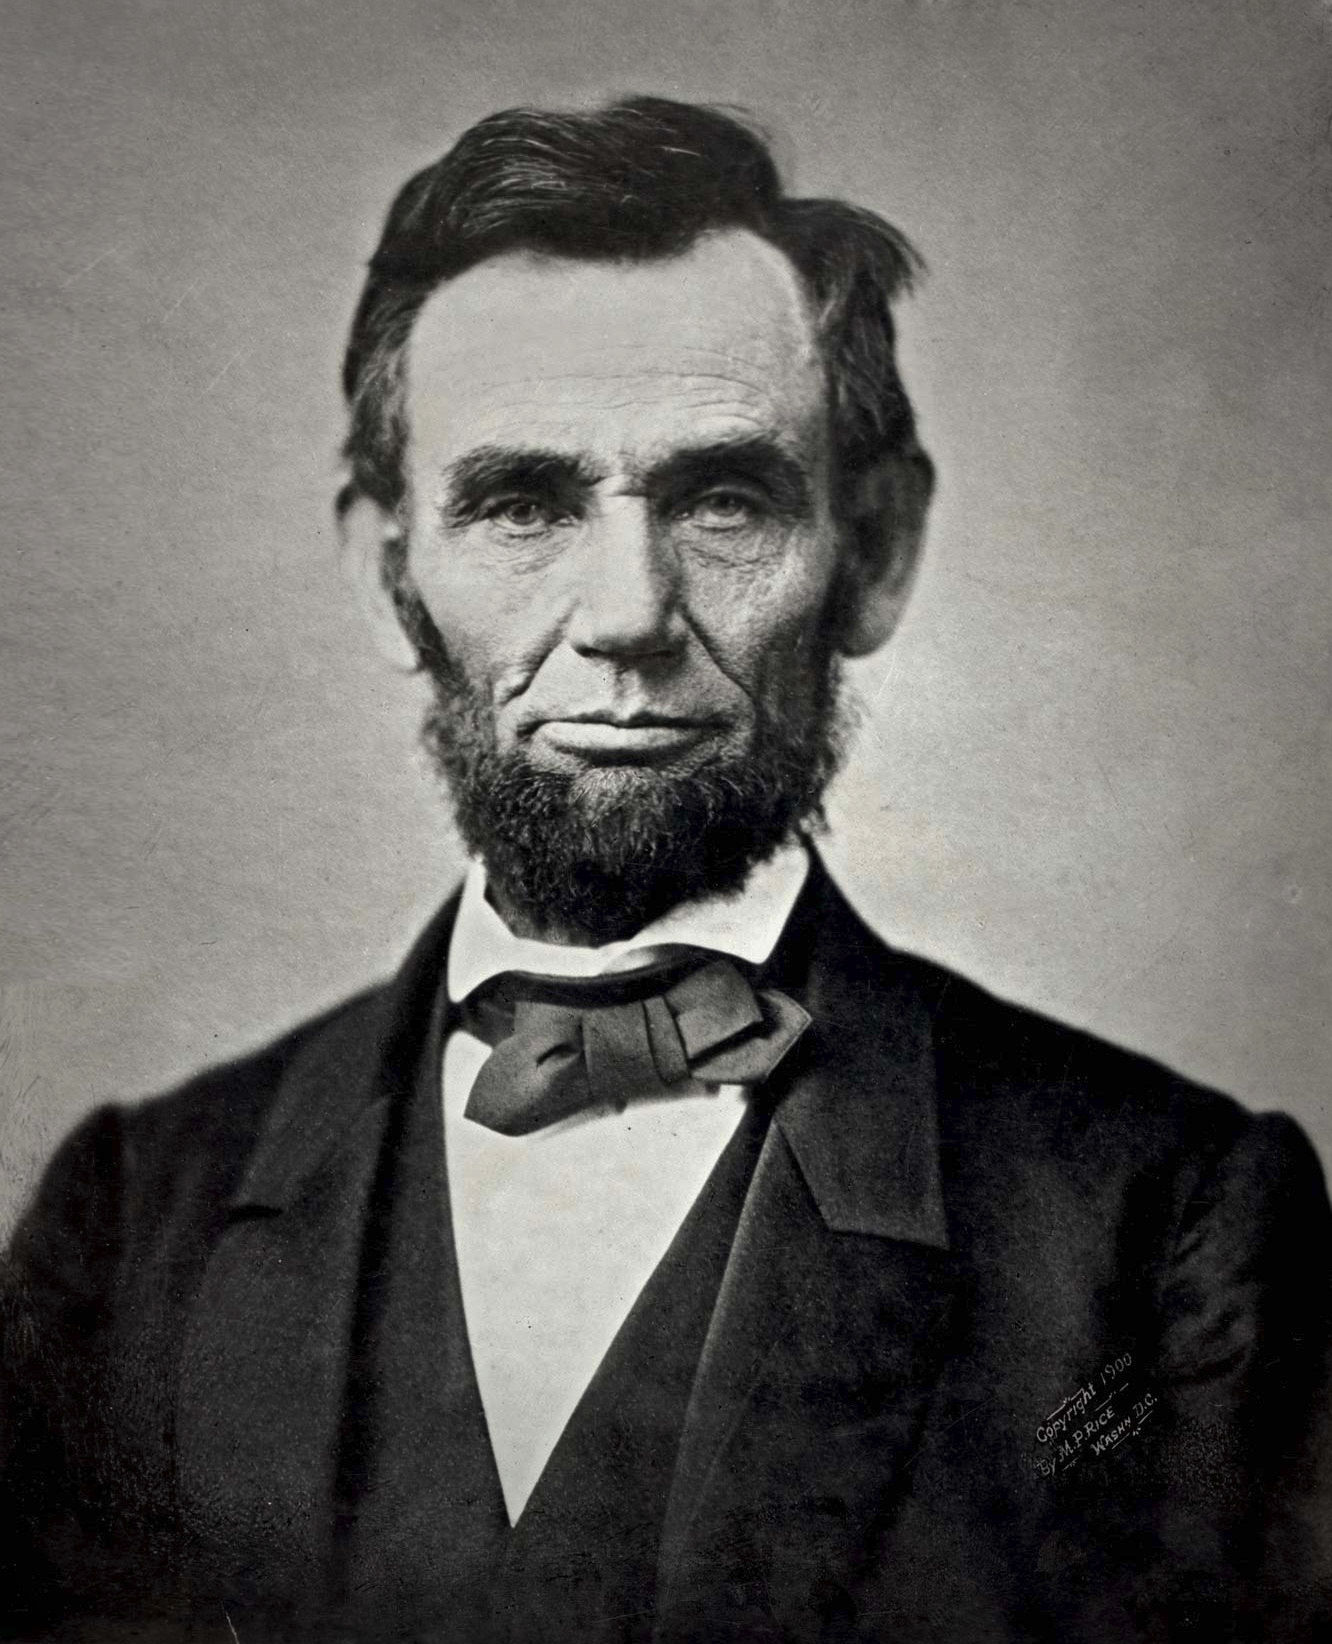
\includegraphics[width=0.5\linewidth]{pix/Abraham_Lincoln_November_1863.png}
	\caption{Abraham Lincoln, 1865.}
	\label{fig:AbrahamLincoln}
\end{figure}

\subsection{Multipass Results}
To determine if there are any statistically significant variations in running the same program on the same image multiple times, a script was written to test this condition. For VM, the results of each run using 4000 points, subpixel density 5, non-overlapping, andvariable radius were extremely consistent. Minor variations in the duration of the runs were seen. Over 5 runs, times ranged from 56.78 seconds for

\begin{figure}[H]
	\centering
	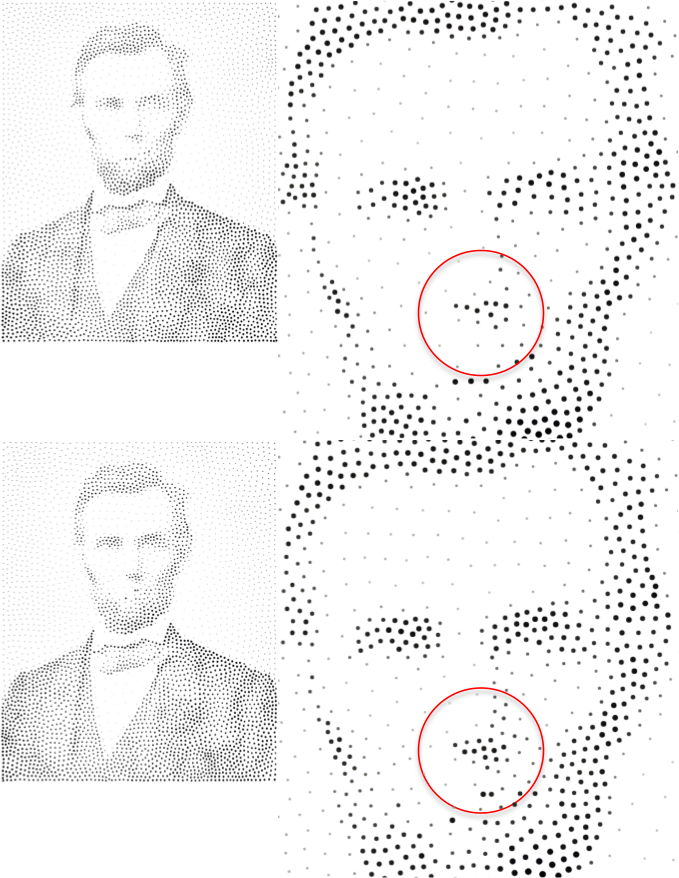
\includegraphics[width=0.5\linewidth]{pix/2-1_hc_differences.png}
	\caption{Pixel placement differences between hedcuter runs.}
	\label{fig:differences1}
\end{figure}

Figure \ref{fig:differences1} shows the pixel differences between different hedcuter runs.


\begin{figure}[H]
	\centering
	\begin{subfigure}[b]{0.2\linewidth}
		
\includegraphics[width=\linewidth]{pix/hc_AL_1000_r1.png}
		\caption{1000px, r=1}
	\end{subfigure}
	\begin{subfigure}[b]{0.2\linewidth}
		
\includegraphics[width=\linewidth]{pix/hc_AL_2000_r1.png}
		\caption{2000px, r=1}
	\end{subfigure}
	\begin{subfigure}[b]{0.2\linewidth}
		
\includegraphics[width=\linewidth]{pix/hc_AL_4000_r1.png}
		\caption{4000px, r=1}
	\end{subfigure}
	\begin{subfigure}[b]{0.2\linewidth}
		
\includegraphics[width=\linewidth]{pix/hc_AL_8000_r1.png}
		\caption{8000px, r=1}
	\end{subfigure}
	\begin{subfigure}[b]{0.2\linewidth}
		
\includegraphics[width=\linewidth]{pix/hc_AL_1000_r5.png}
		\caption{1000px, r=5}
	\end{subfigure}
	\begin{subfigure}[b]{0.2\linewidth}
		
\includegraphics[width=\linewidth]{pix/hc_AL_2000_r5.png}
		\caption{2000px, r=5}
	\end{subfigure}
	\begin{subfigure}[b]{0.2\linewidth}
		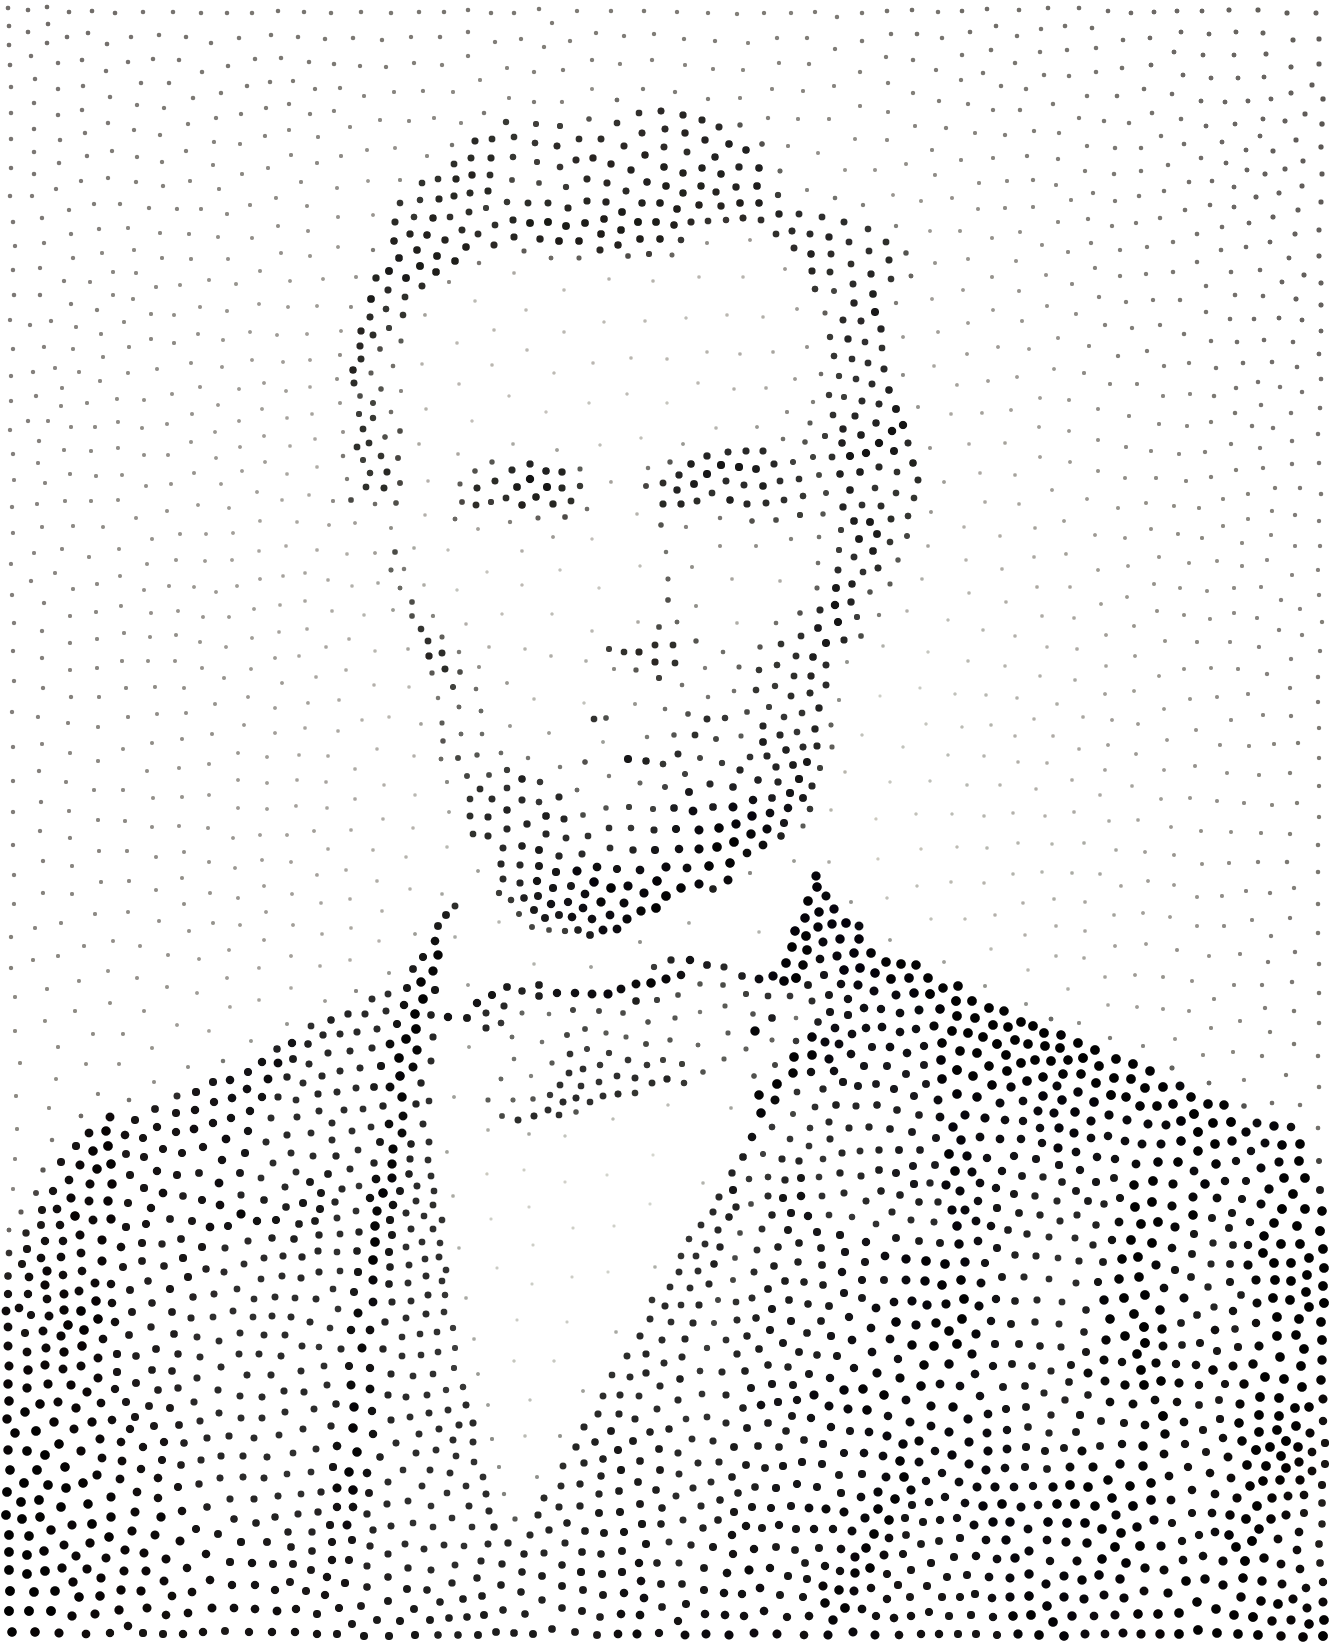
\includegraphics[width=\linewidth]{pix/hc_AL_4000_r5.png}
		\caption{4000px, r=5}
	\end{subfigure}
	\begin{subfigure}[b]{0.2\linewidth}
		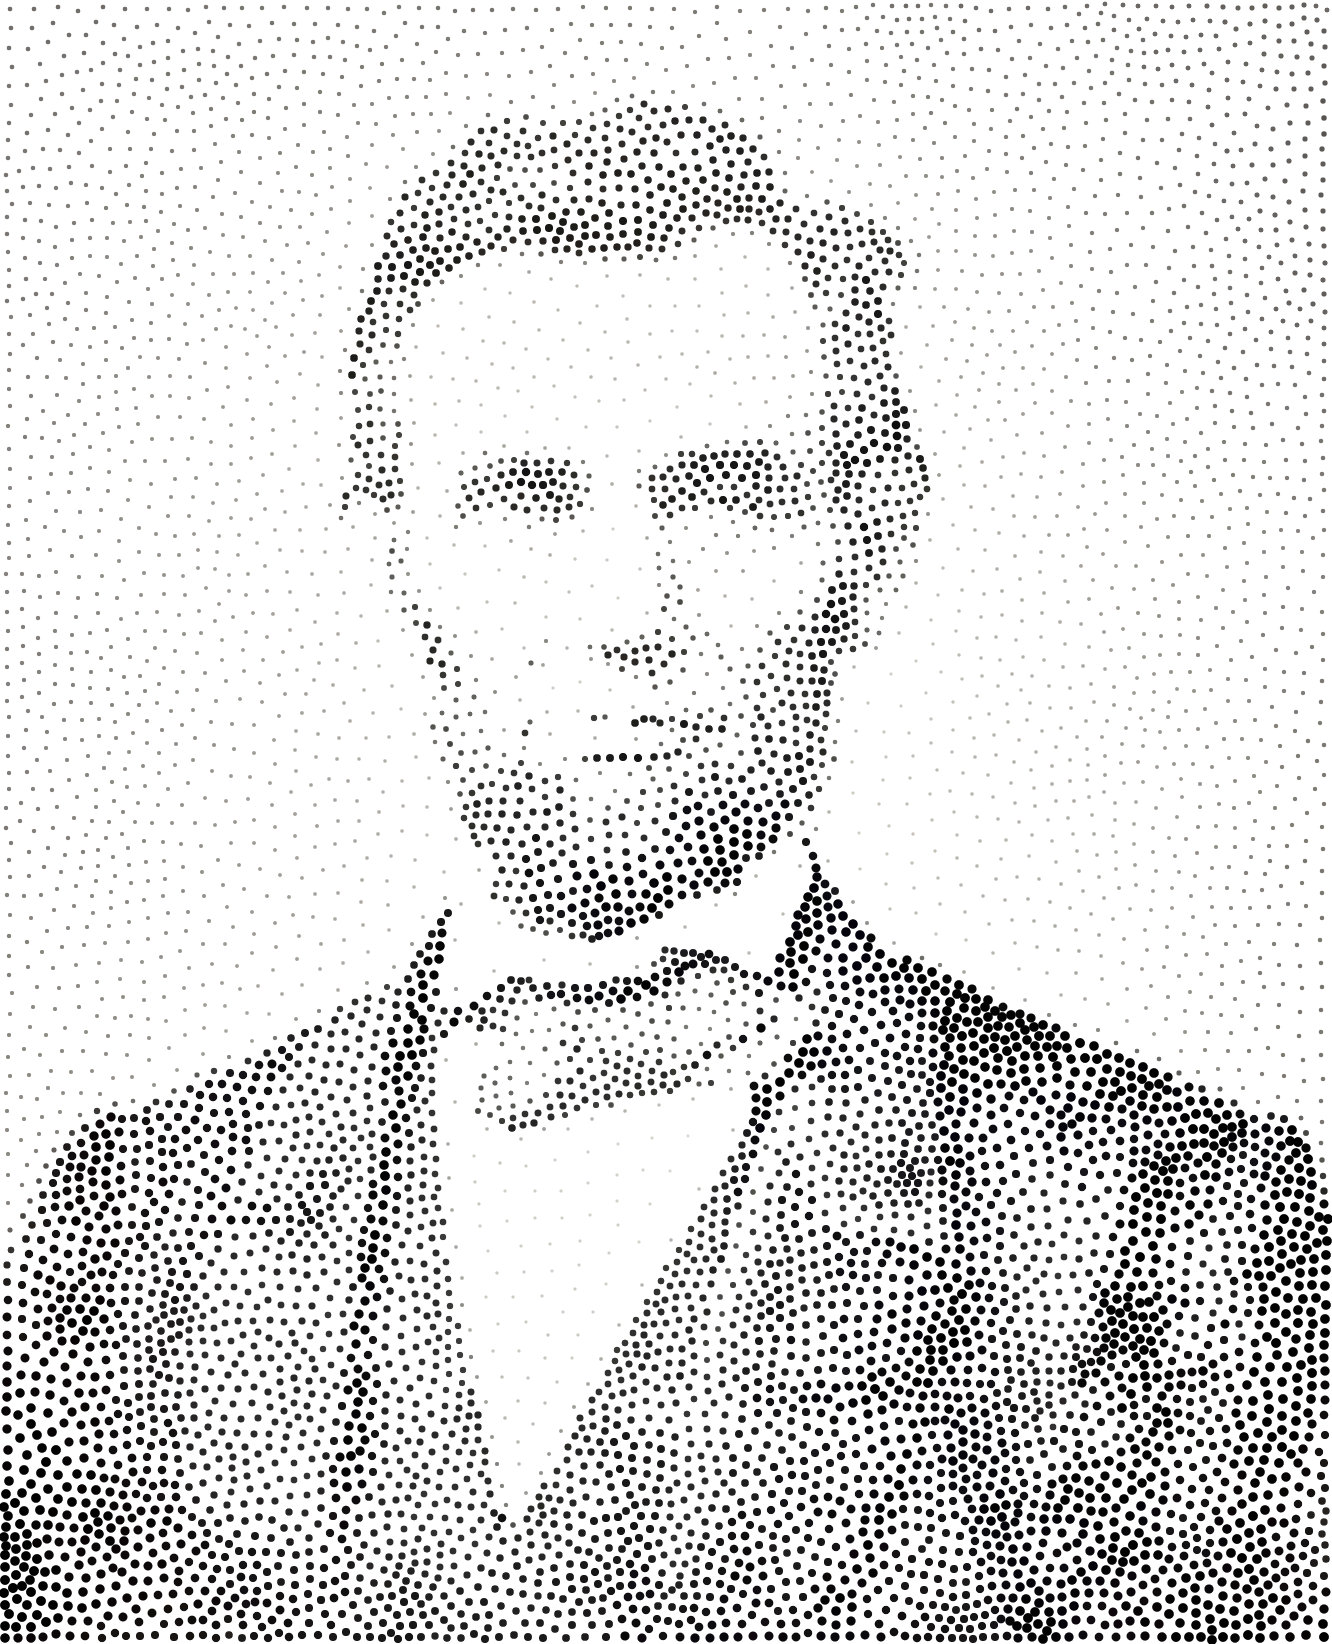
\includegraphics[width=\linewidth]{pix/hc_AL_8000_r5.png}
		\caption{8000px, r=5}
	\end{subfigure}
	\begin{subfigure}[b]{0.2\linewidth}
		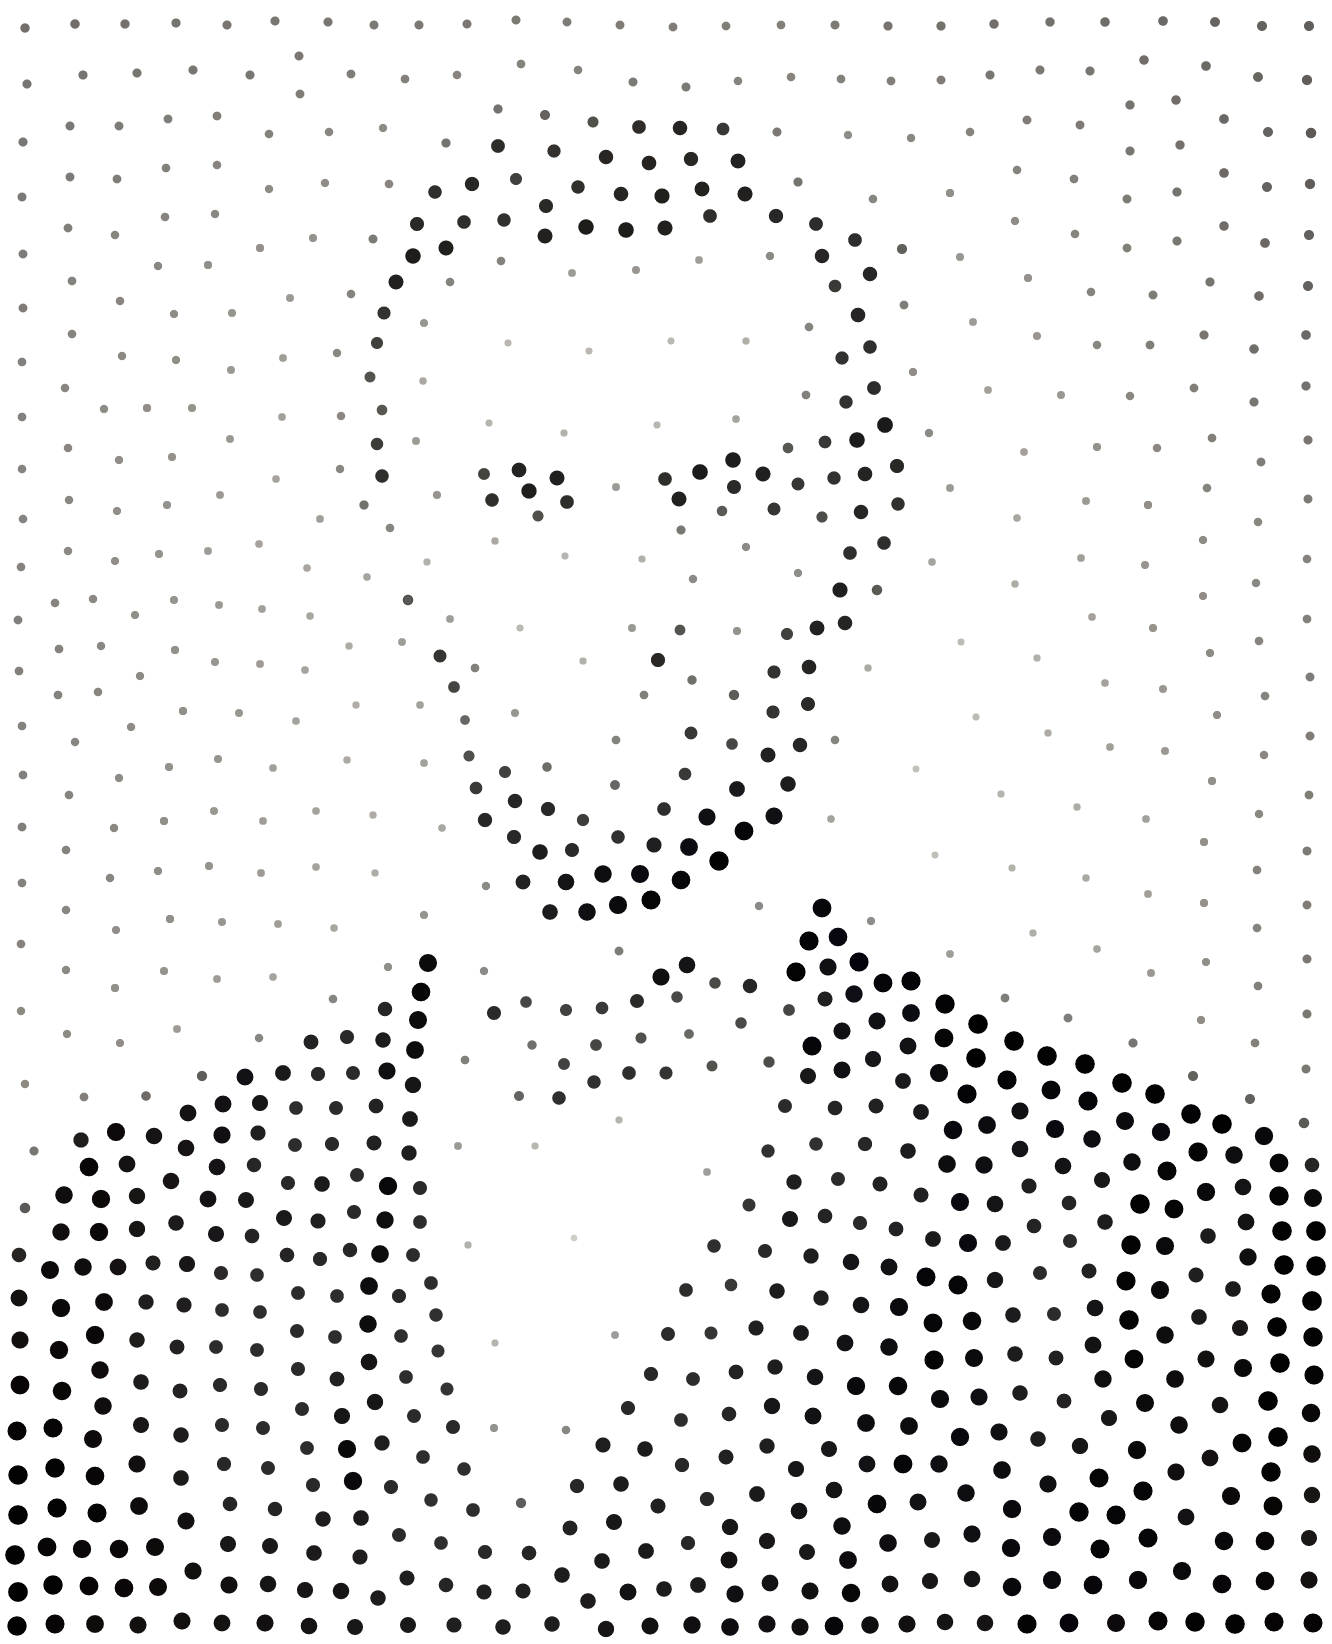
\includegraphics[width=\linewidth]{pix/hc_AL_1000_r10.png}
		\caption{1000px, r=10}
	\end{subfigure}
	\begin{subfigure}[b]{0.2\linewidth}
		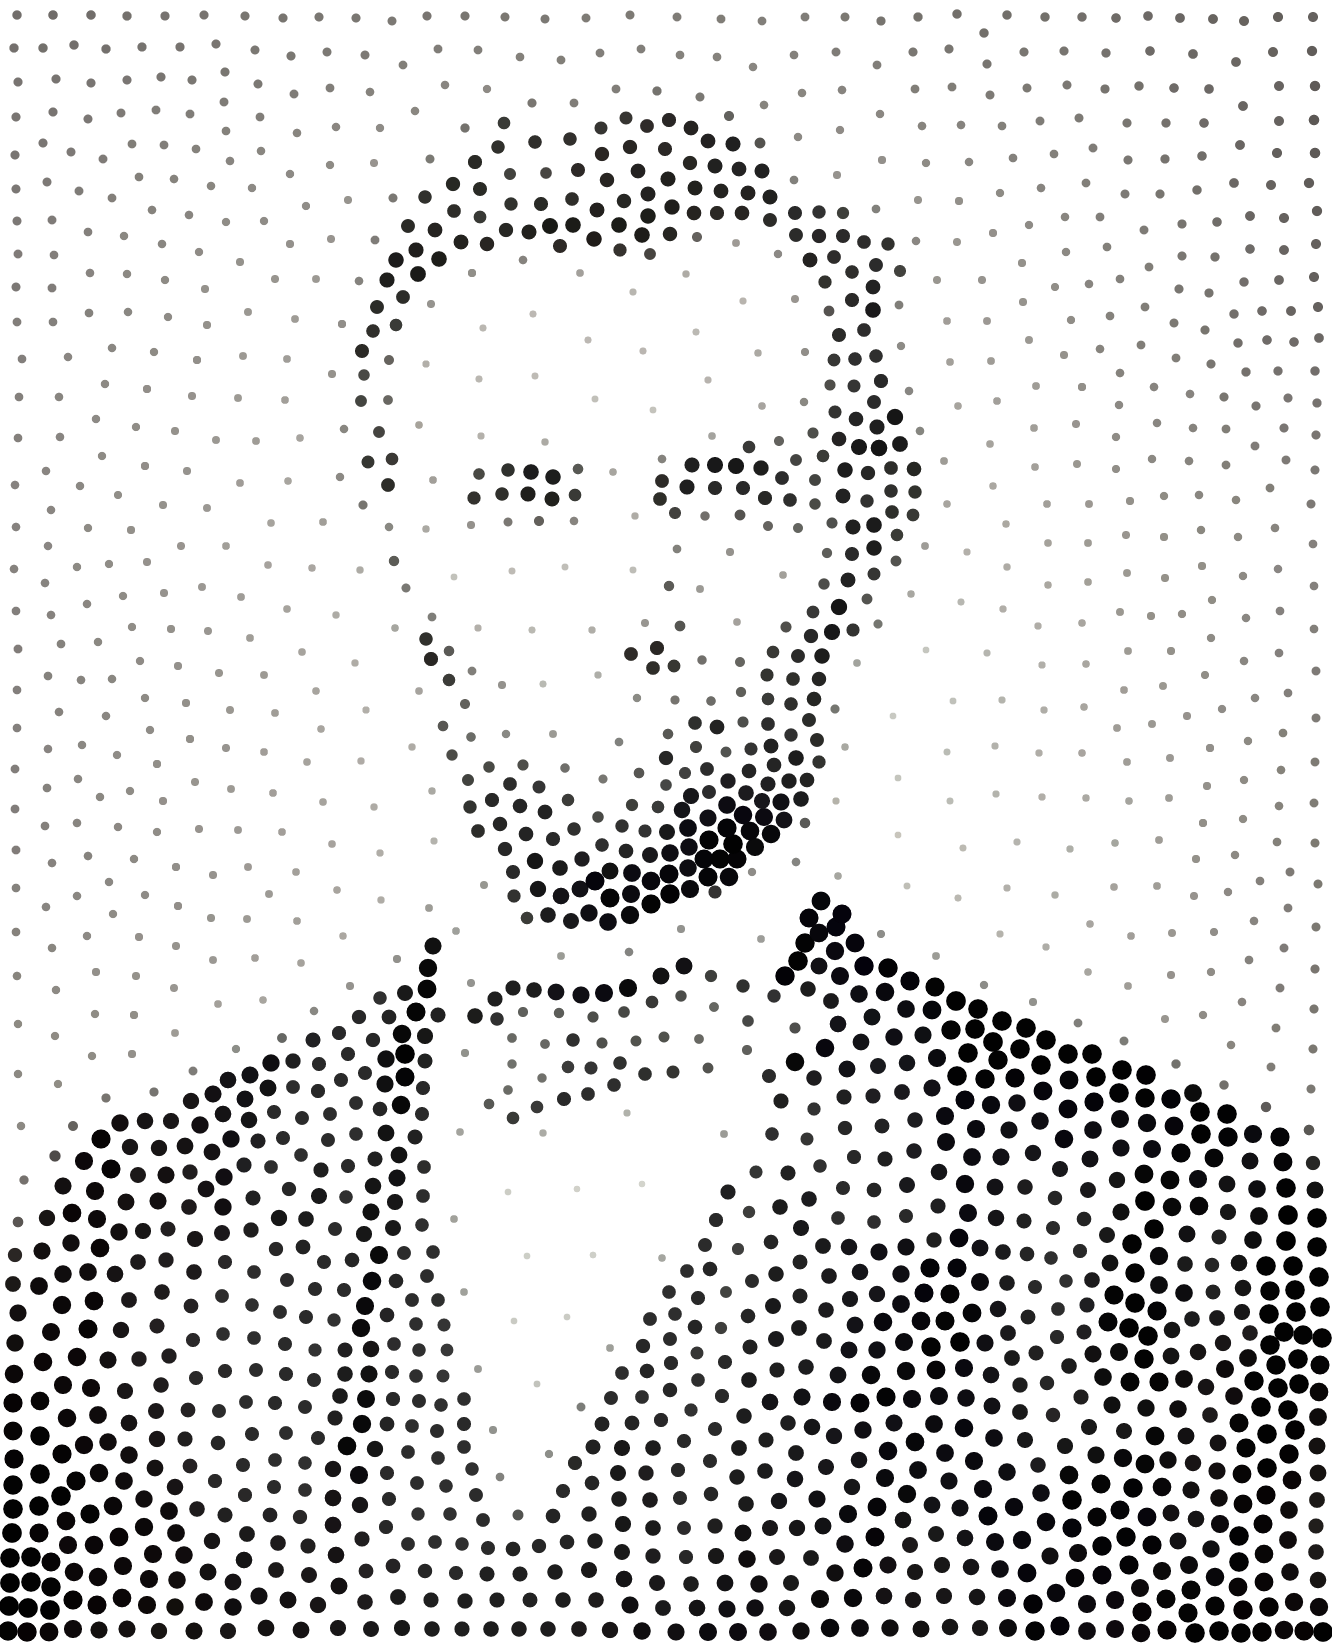
\includegraphics[width=\linewidth]{pix/hc_AL_2000_r10.png}
		\caption{2000px, r=10}
	\end{subfigure}
	\begin{subfigure}[b]{0.2\linewidth}
		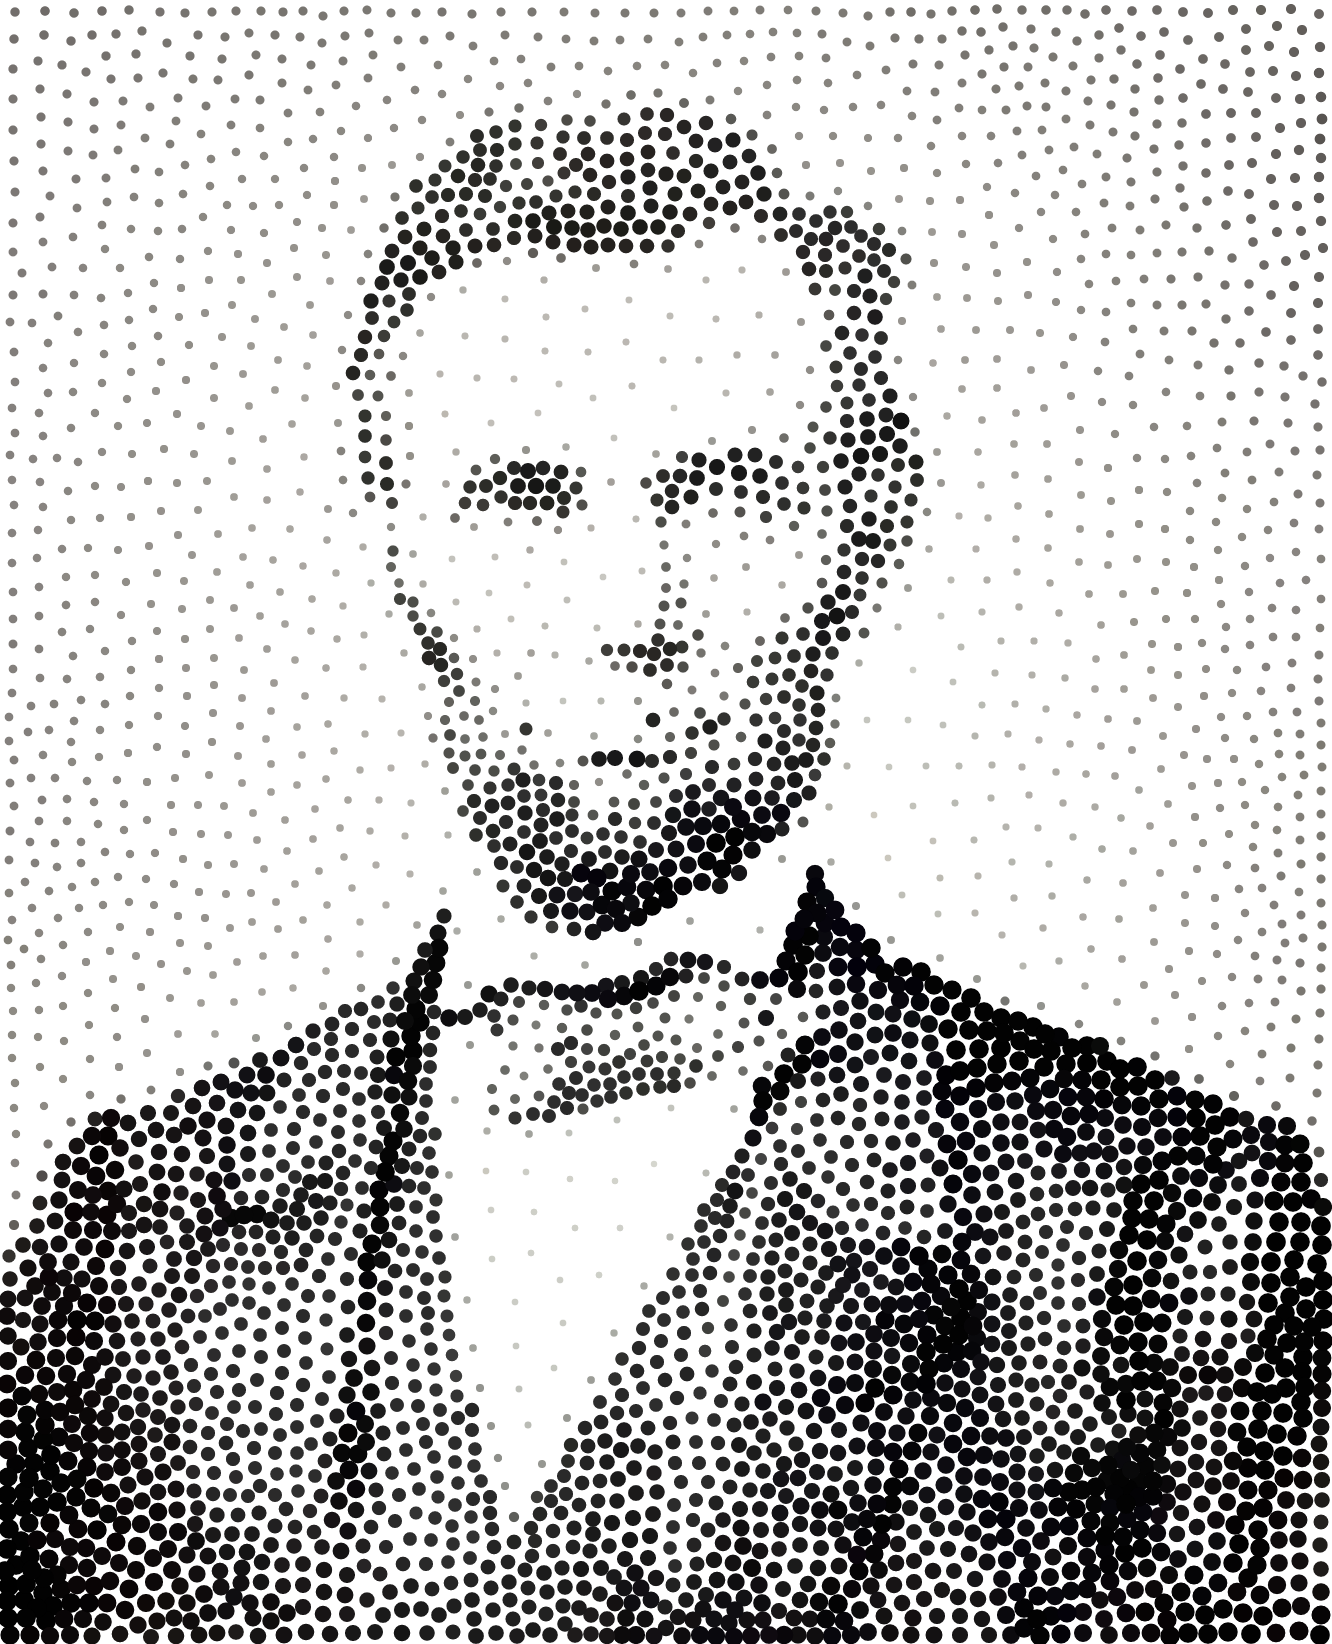
\includegraphics[width=\linewidth]{pix/hc_AL_4000_r10.png}
		\caption{4000px, r=10}
	\end{subfigure}
	\begin{subfigure}[b]{0.2\linewidth}
		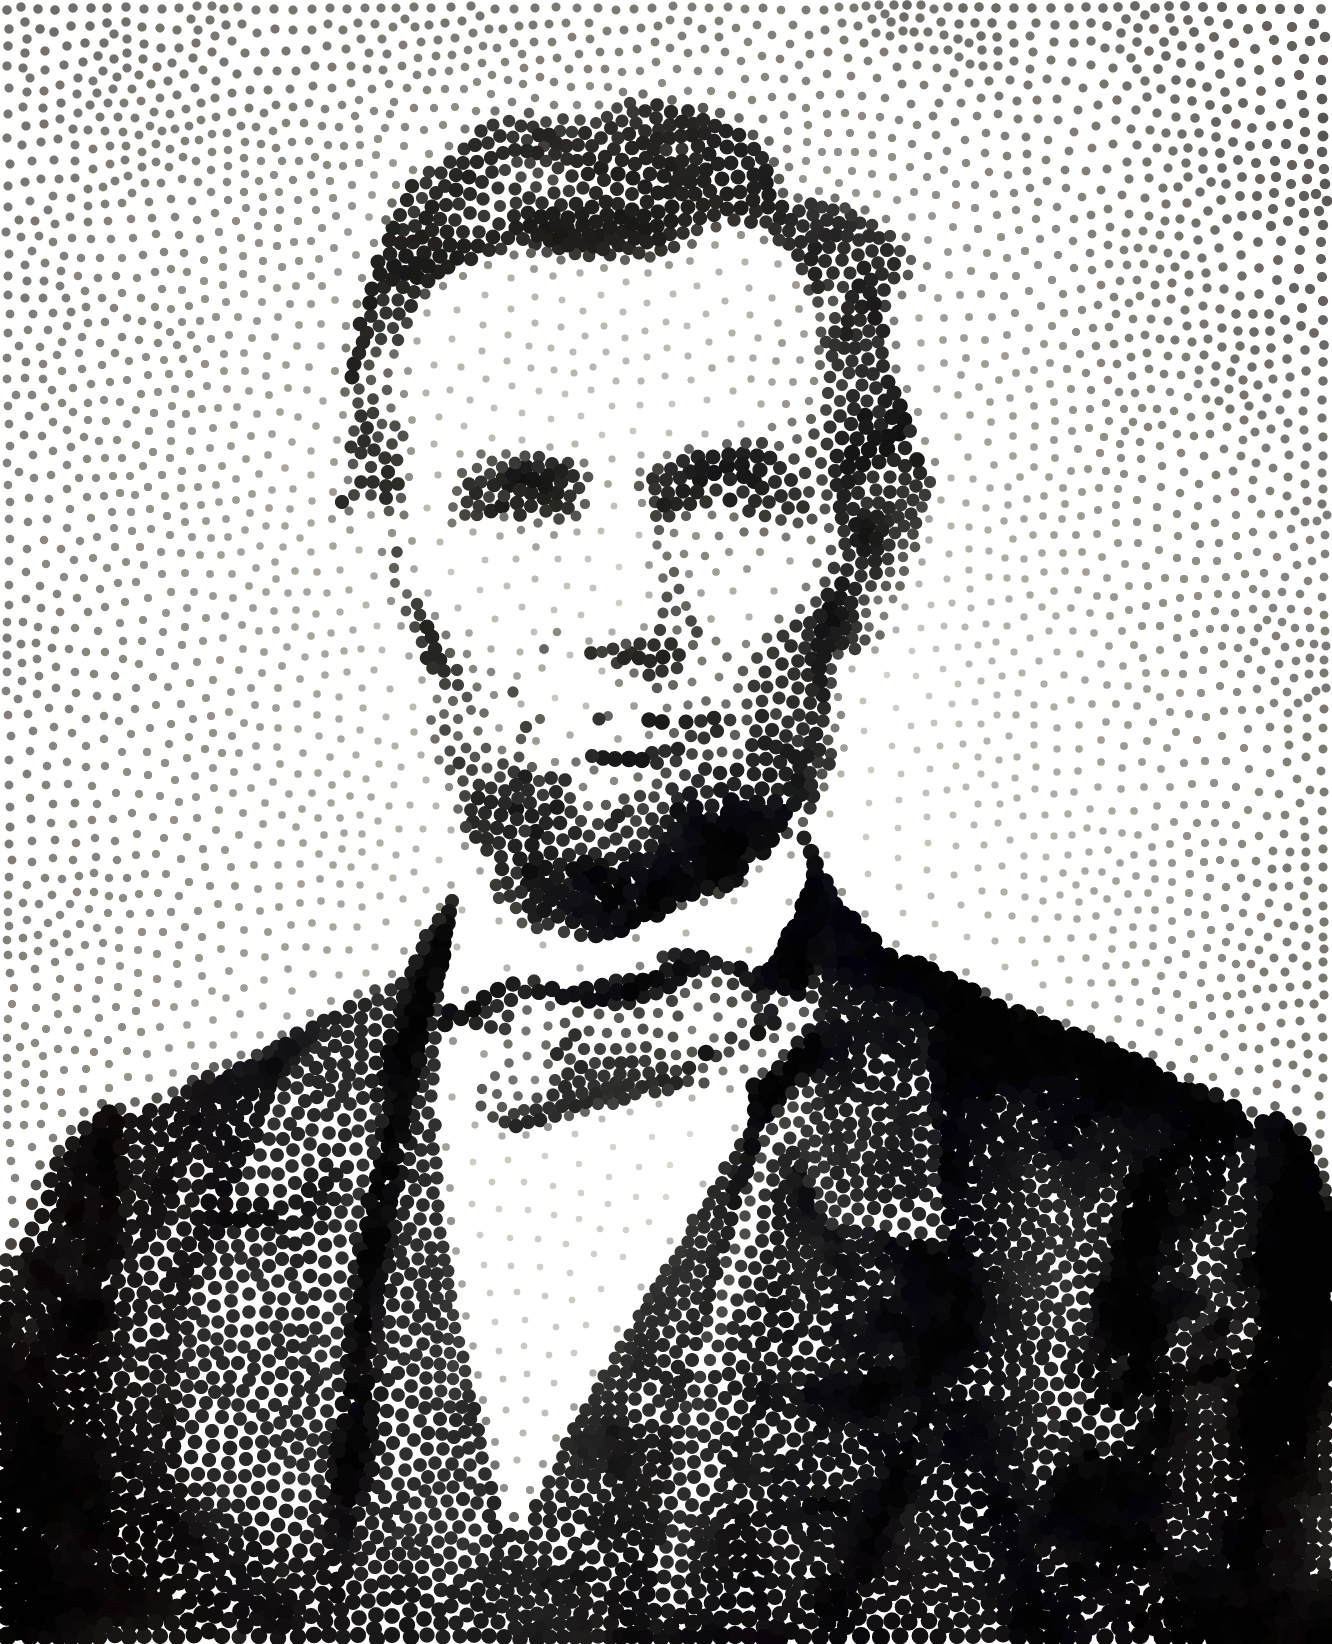
\includegraphics[width=\linewidth]{pix/hc_AL_8000_r10.png}
		\caption{8000px, r=10}
	\end{subfigure}
	\caption{Hedcuter images varying number of disks. Radius = 1.}
	\label{fig:hc_points1}
\end{figure}

\begin{figure}[H]
	\centering
	\begin{subfigure}[b]{0.2\linewidth}
		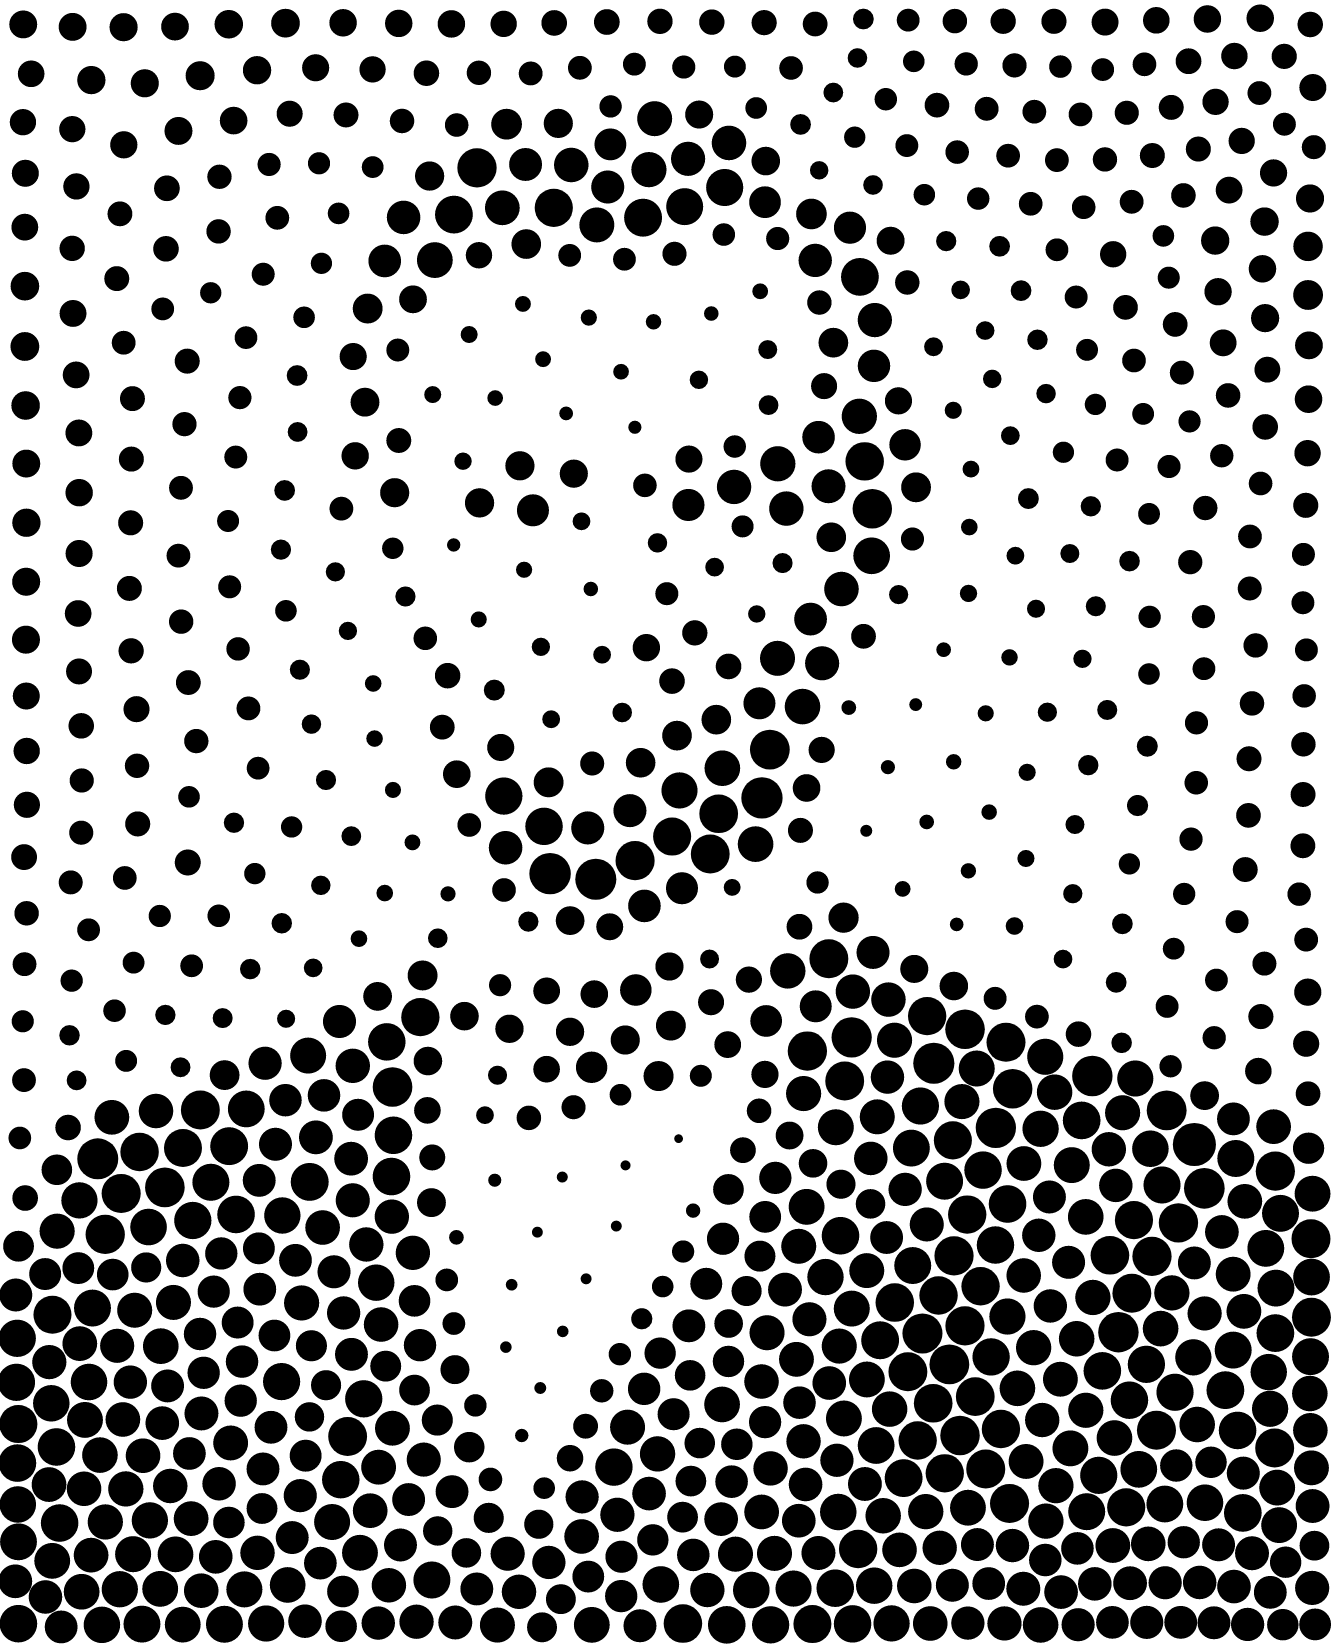
\includegraphics[width=\linewidth]{pix/vr_AL_1000_r1.png}
		\caption{1000px, r=1}
	\end{subfigure}
	\begin{subfigure}[b]{0.2\linewidth}
		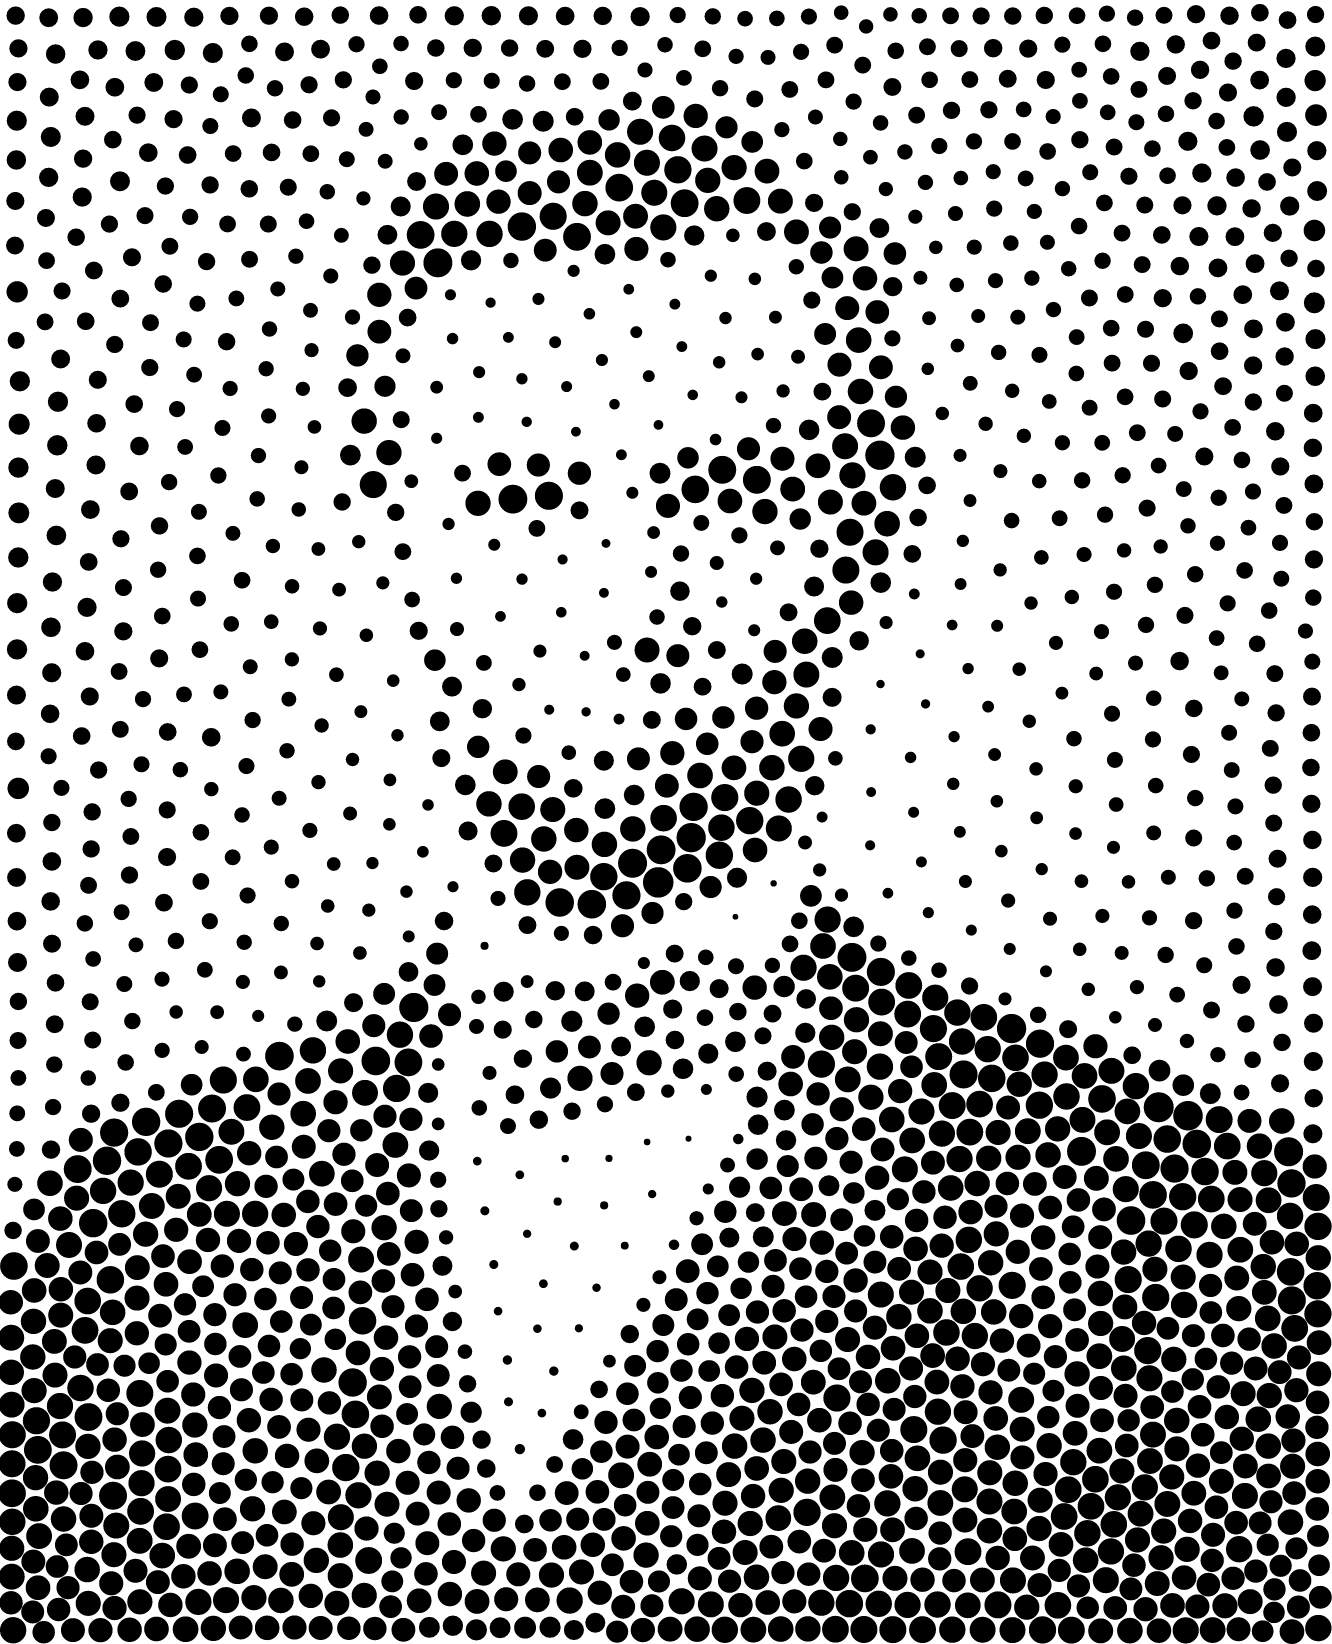
\includegraphics[width=\linewidth]{pix/vr_AL_2000_r1.png}
		\caption{2000px, r=1}
	\end{subfigure}
	\begin{subfigure}[b]{0.2\linewidth}
		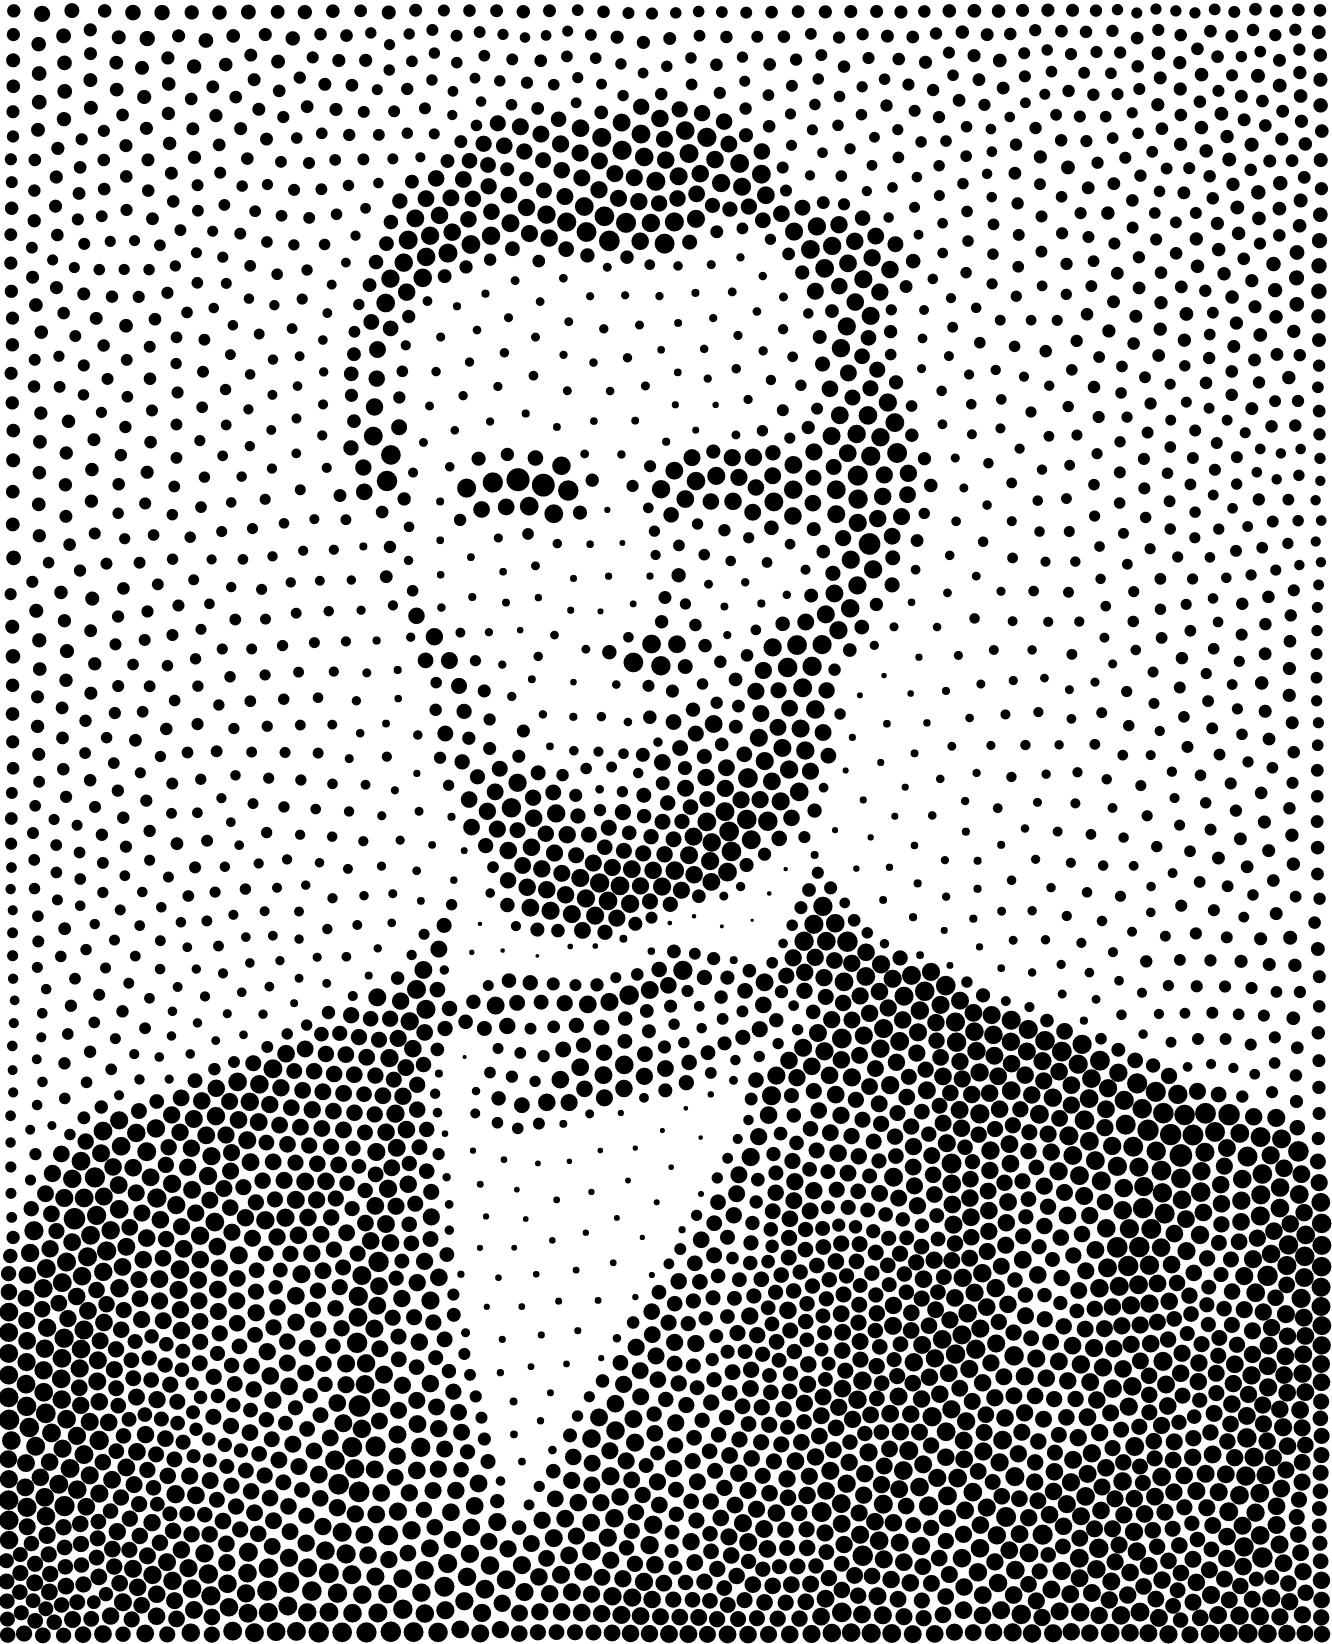
\includegraphics[width=\linewidth]{pix/vr_AL_4000_r1.png}
		\caption{4000px, r=1}
	\end{subfigure}
	\begin{subfigure}[b]{0.2\linewidth}
		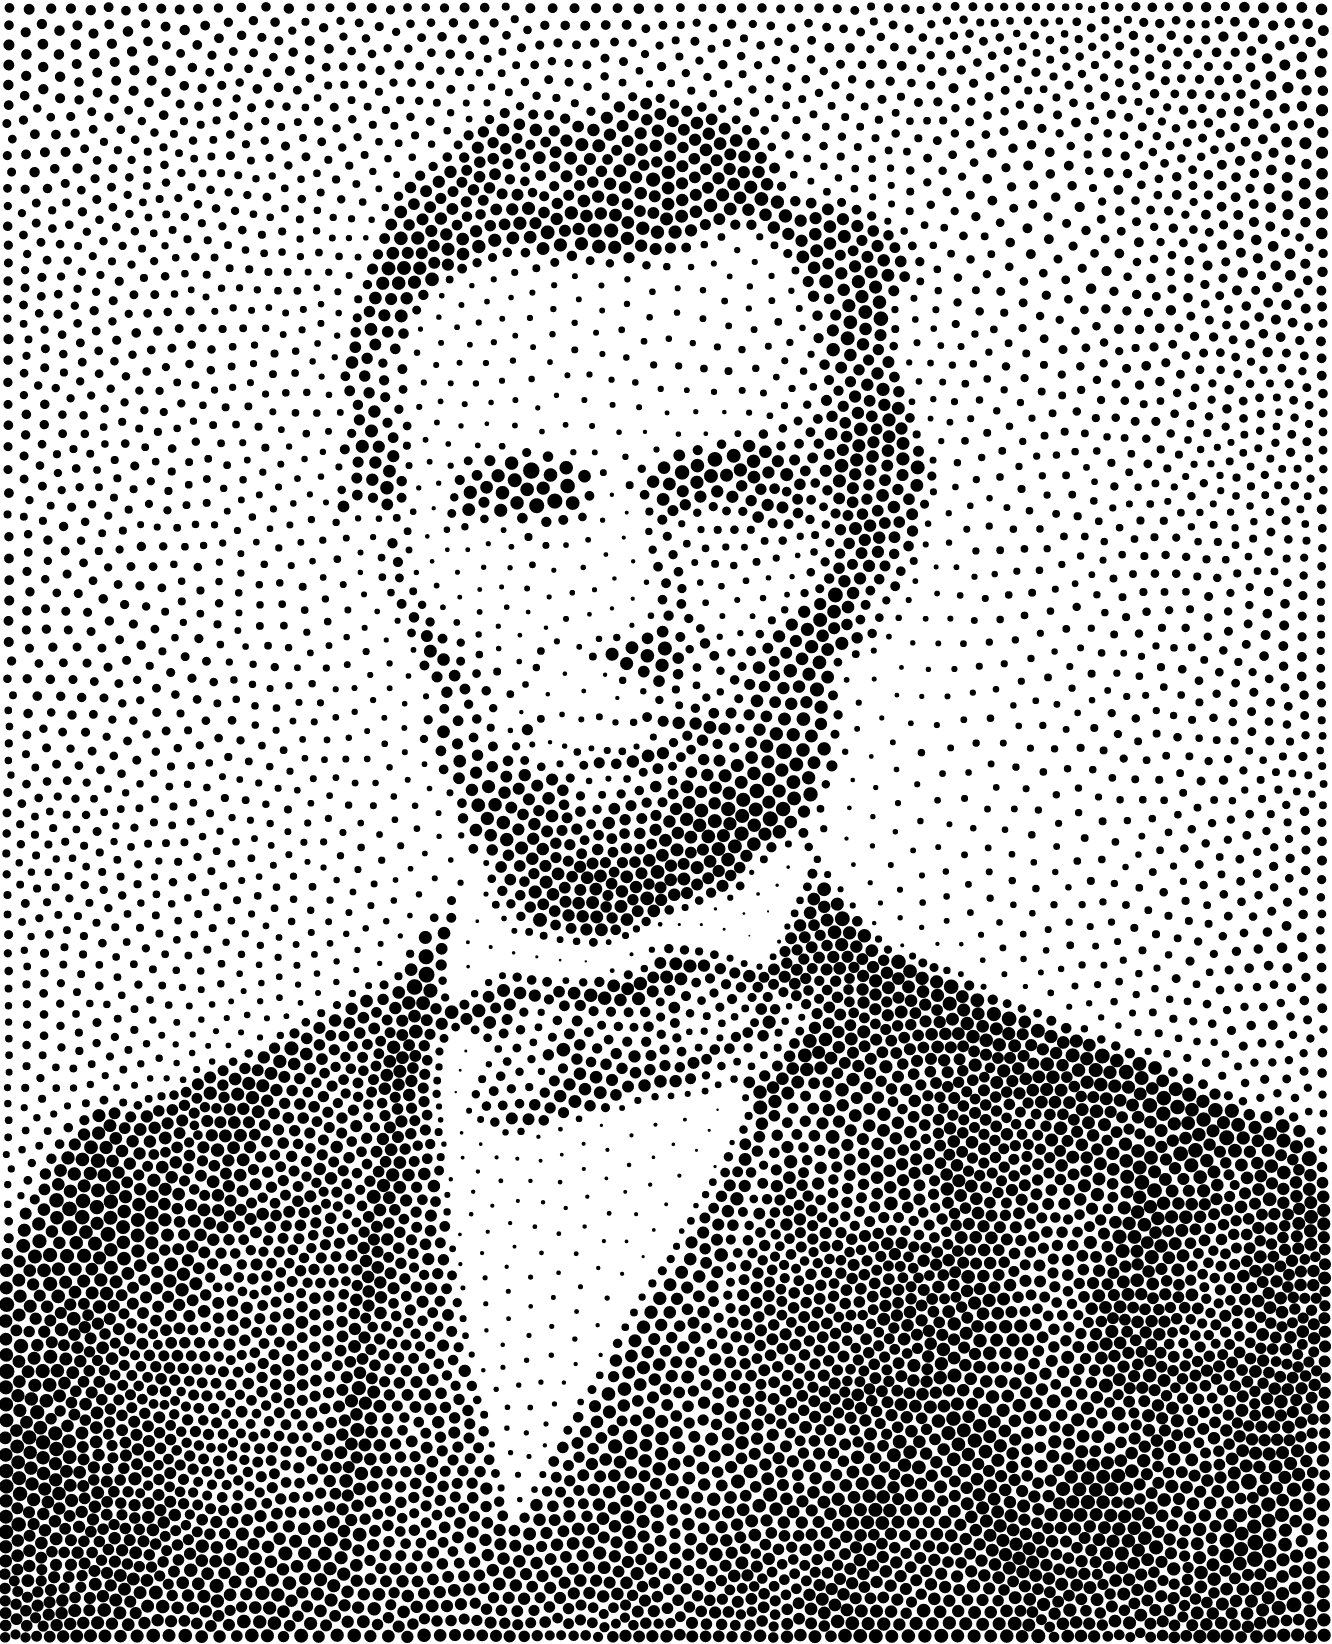
\includegraphics[width=\linewidth]{pix/vr_AL_8000_r1.png}
		\caption{8000px, r=1}
	\end{subfigure}
	\begin{subfigure}[b]{0.2\linewidth}
		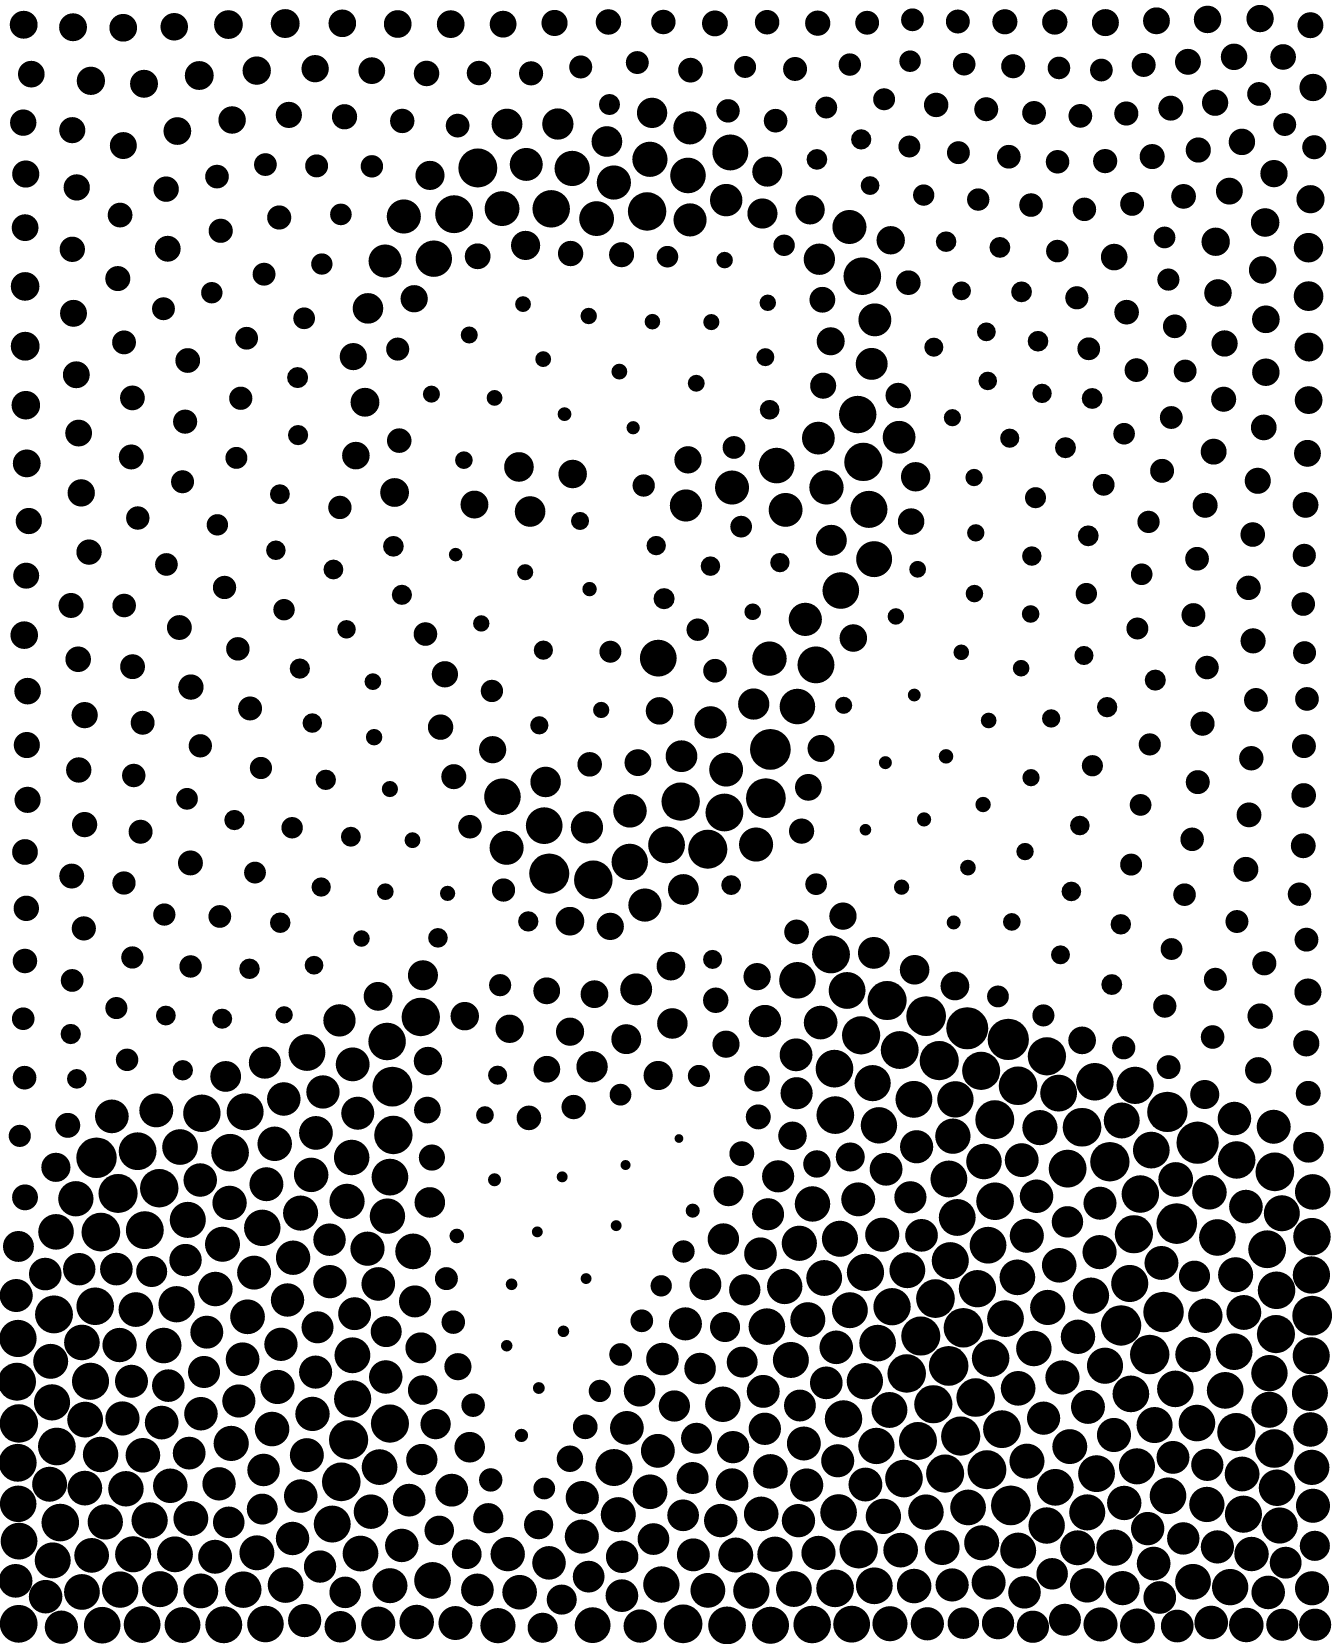
\includegraphics[width=\linewidth]{pix/vr_AL_1000_r5.png}
		\caption{1000px, r=5}
	\end{subfigure}
	\begin{subfigure}[b]{0.2\linewidth}
		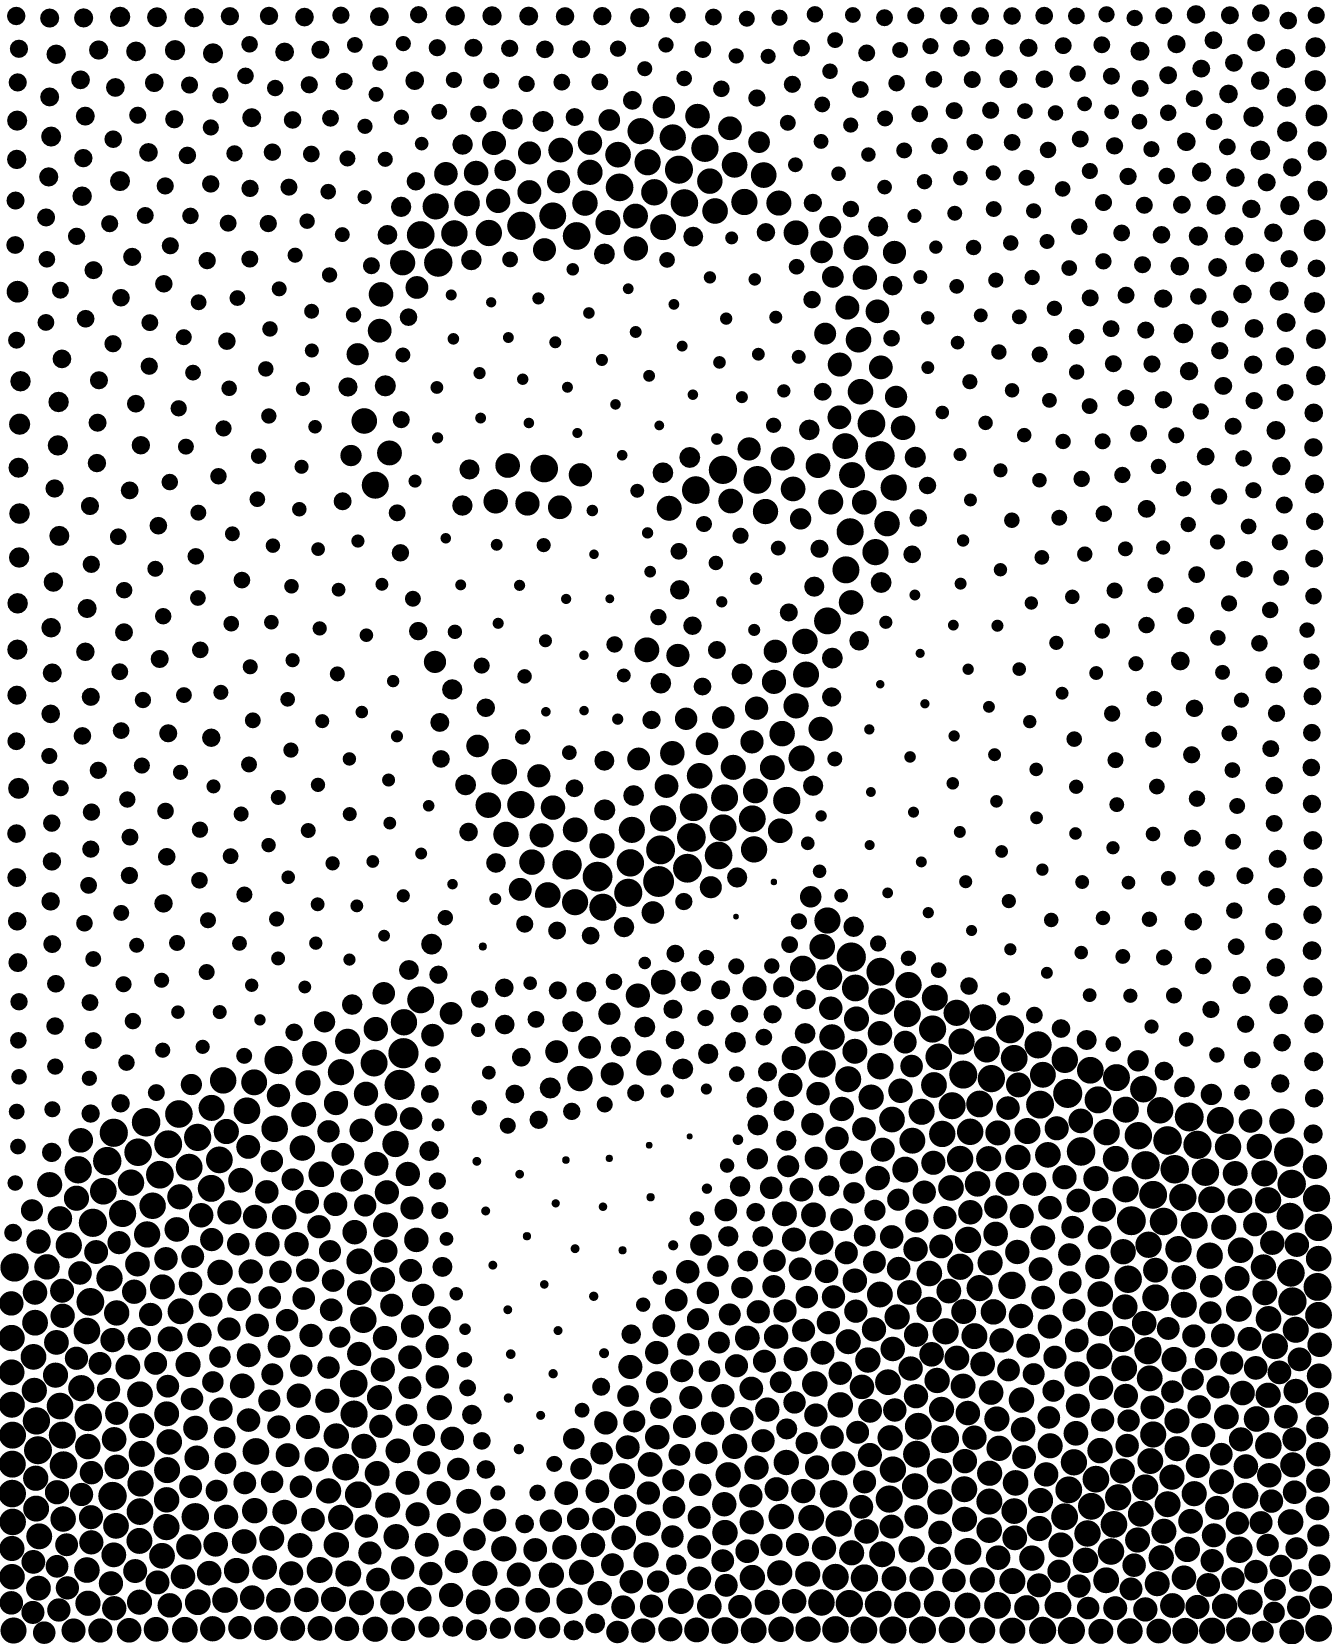
\includegraphics[width=\linewidth]{pix/vr_AL_2000_r5.png}
		\caption{2000px, r=5}
	\end{subfigure}
	\begin{subfigure}[b]{0.2\linewidth}
		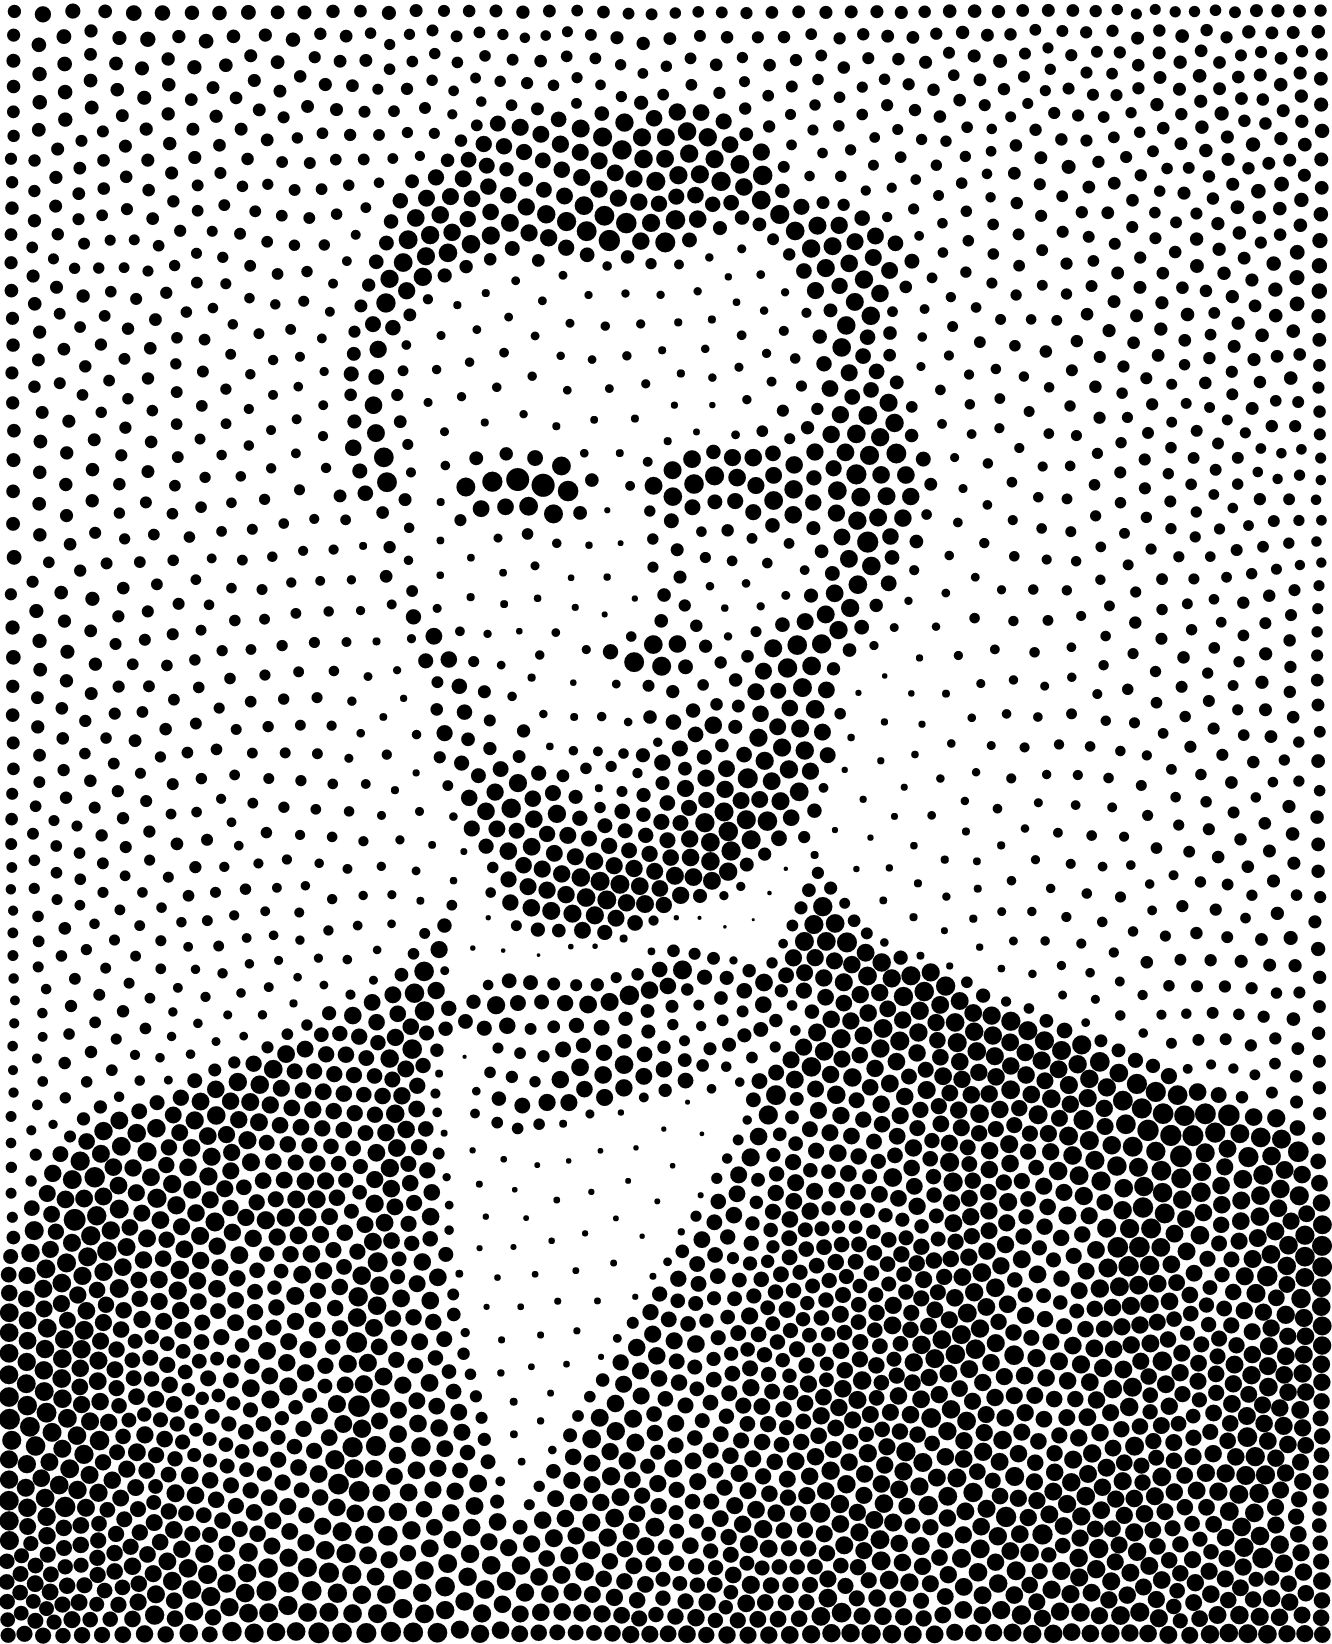
\includegraphics[width=\linewidth]{pix/vr_AL_4000_r5.png}
		\caption{4000px, r=5}
	\end{subfigure}
	\begin{subfigure}[b]{0.2\linewidth}
		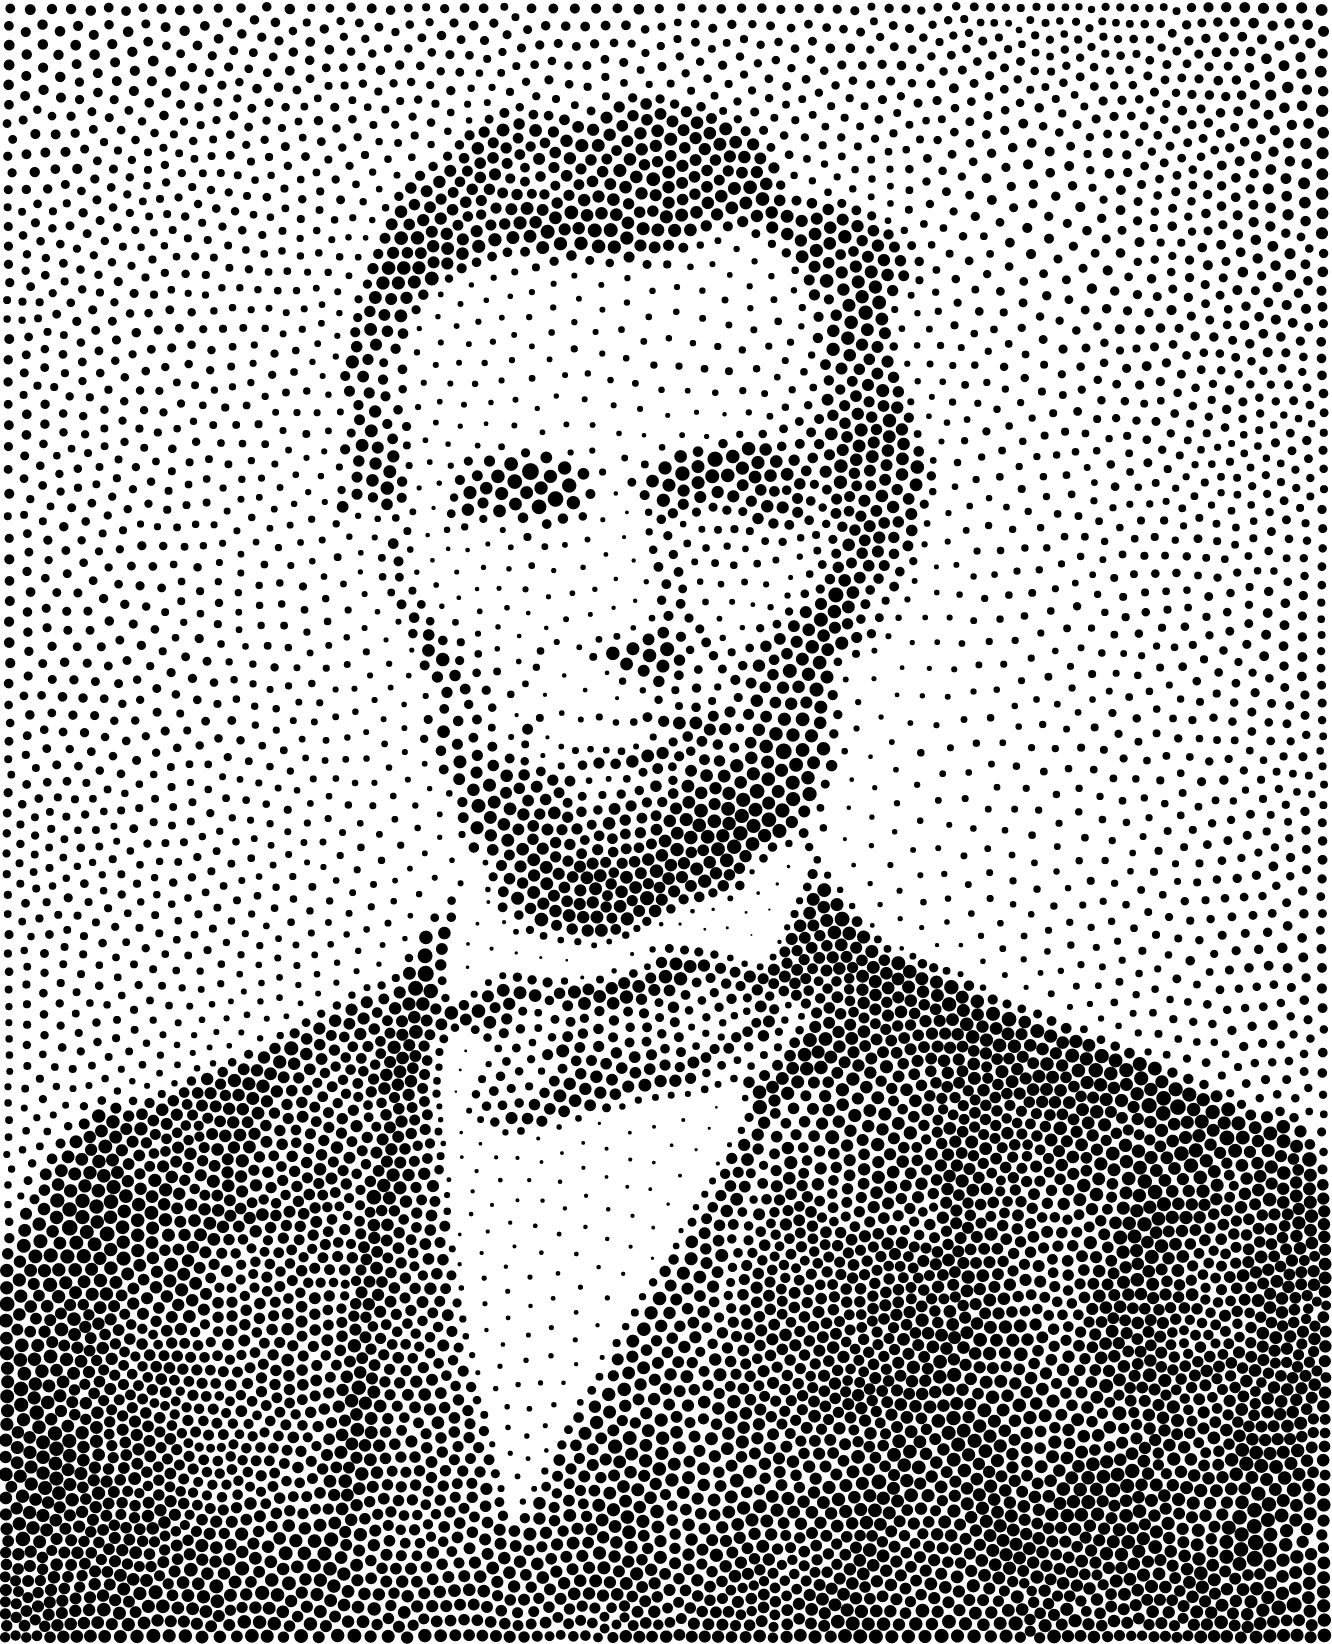
\includegraphics[width=\linewidth]{pix/vr_AL_8000_r5.png}
		\caption{8000px, r=5}
	\end{subfigure}
	\begin{subfigure}[b]{0.2\linewidth}
		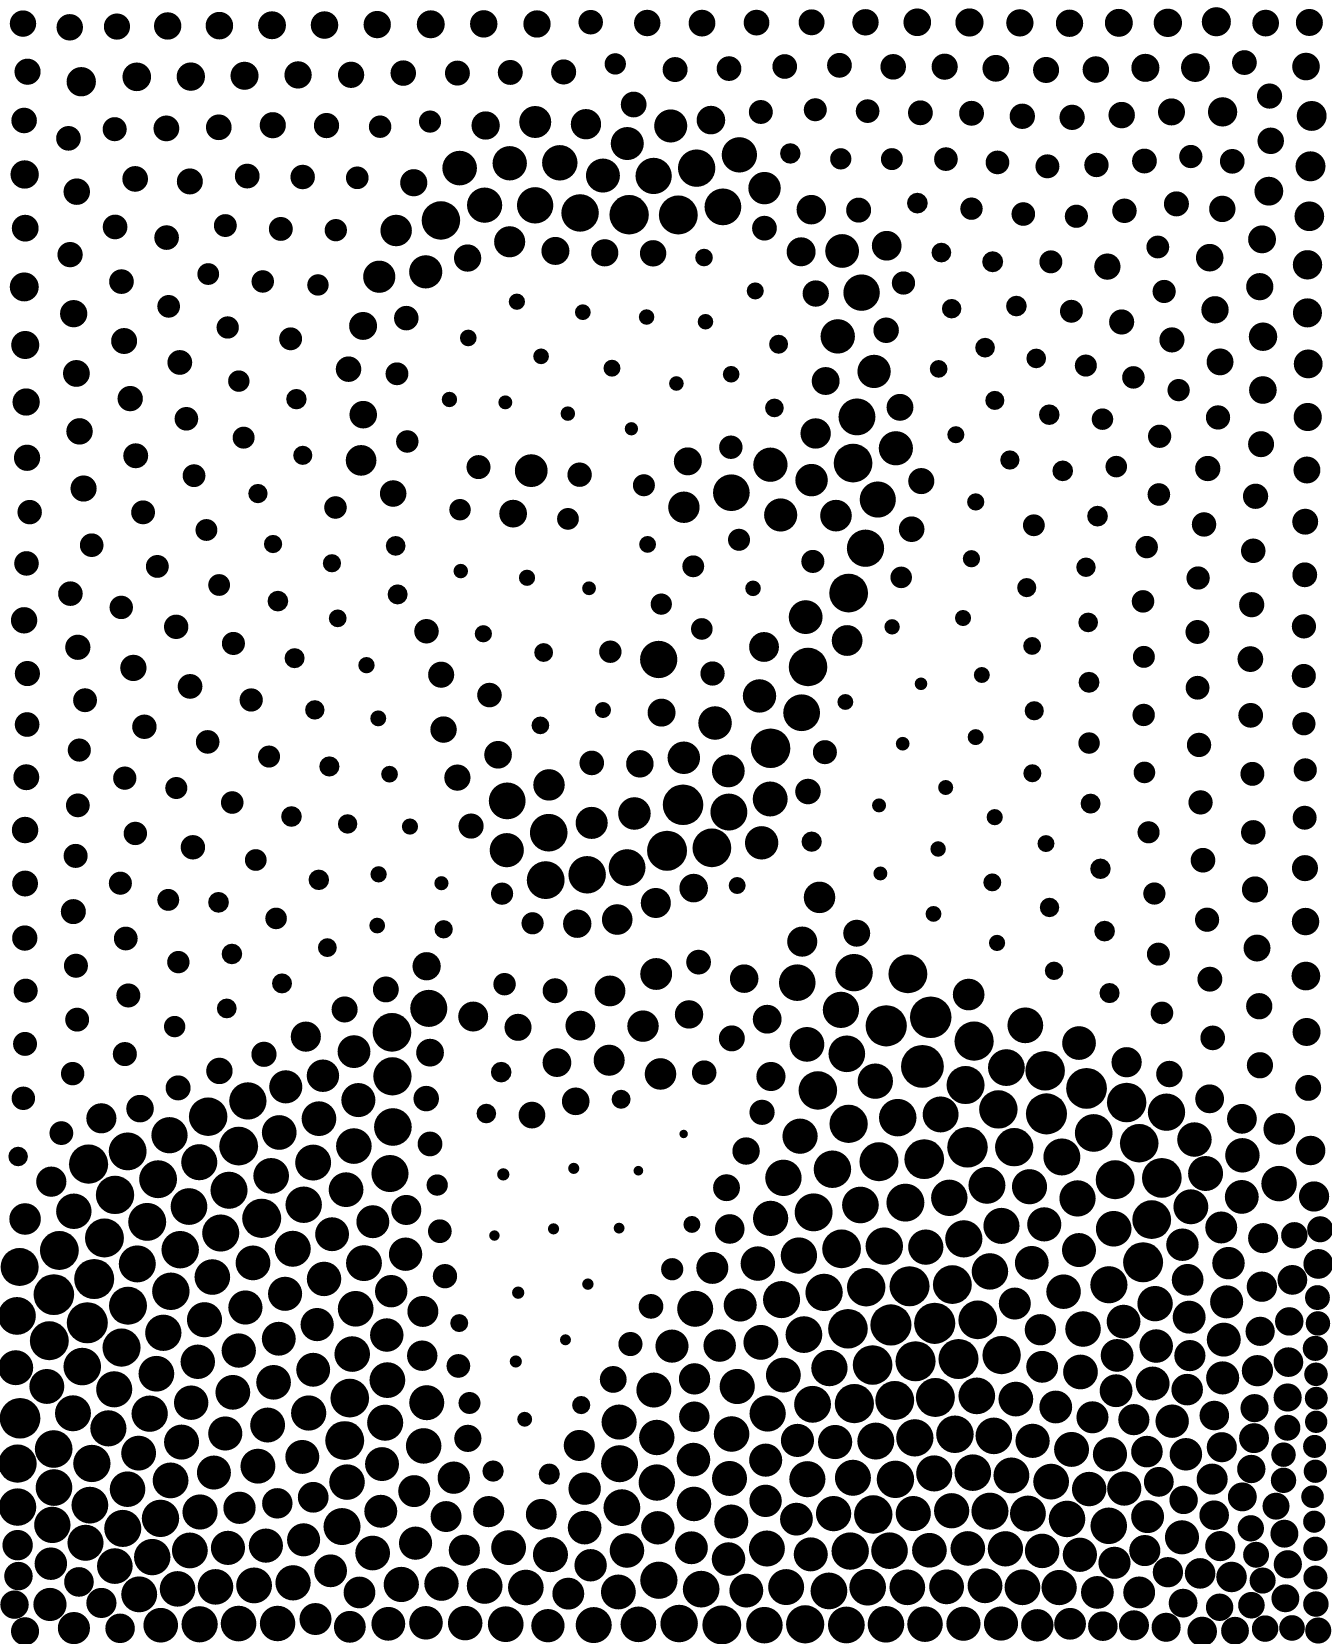
\includegraphics[width=\linewidth]{pix/vr_AL_1000_r10.png}
		\caption{1000px, r=10}
	\end{subfigure}
	\begin{subfigure}[b]{0.2\linewidth}
		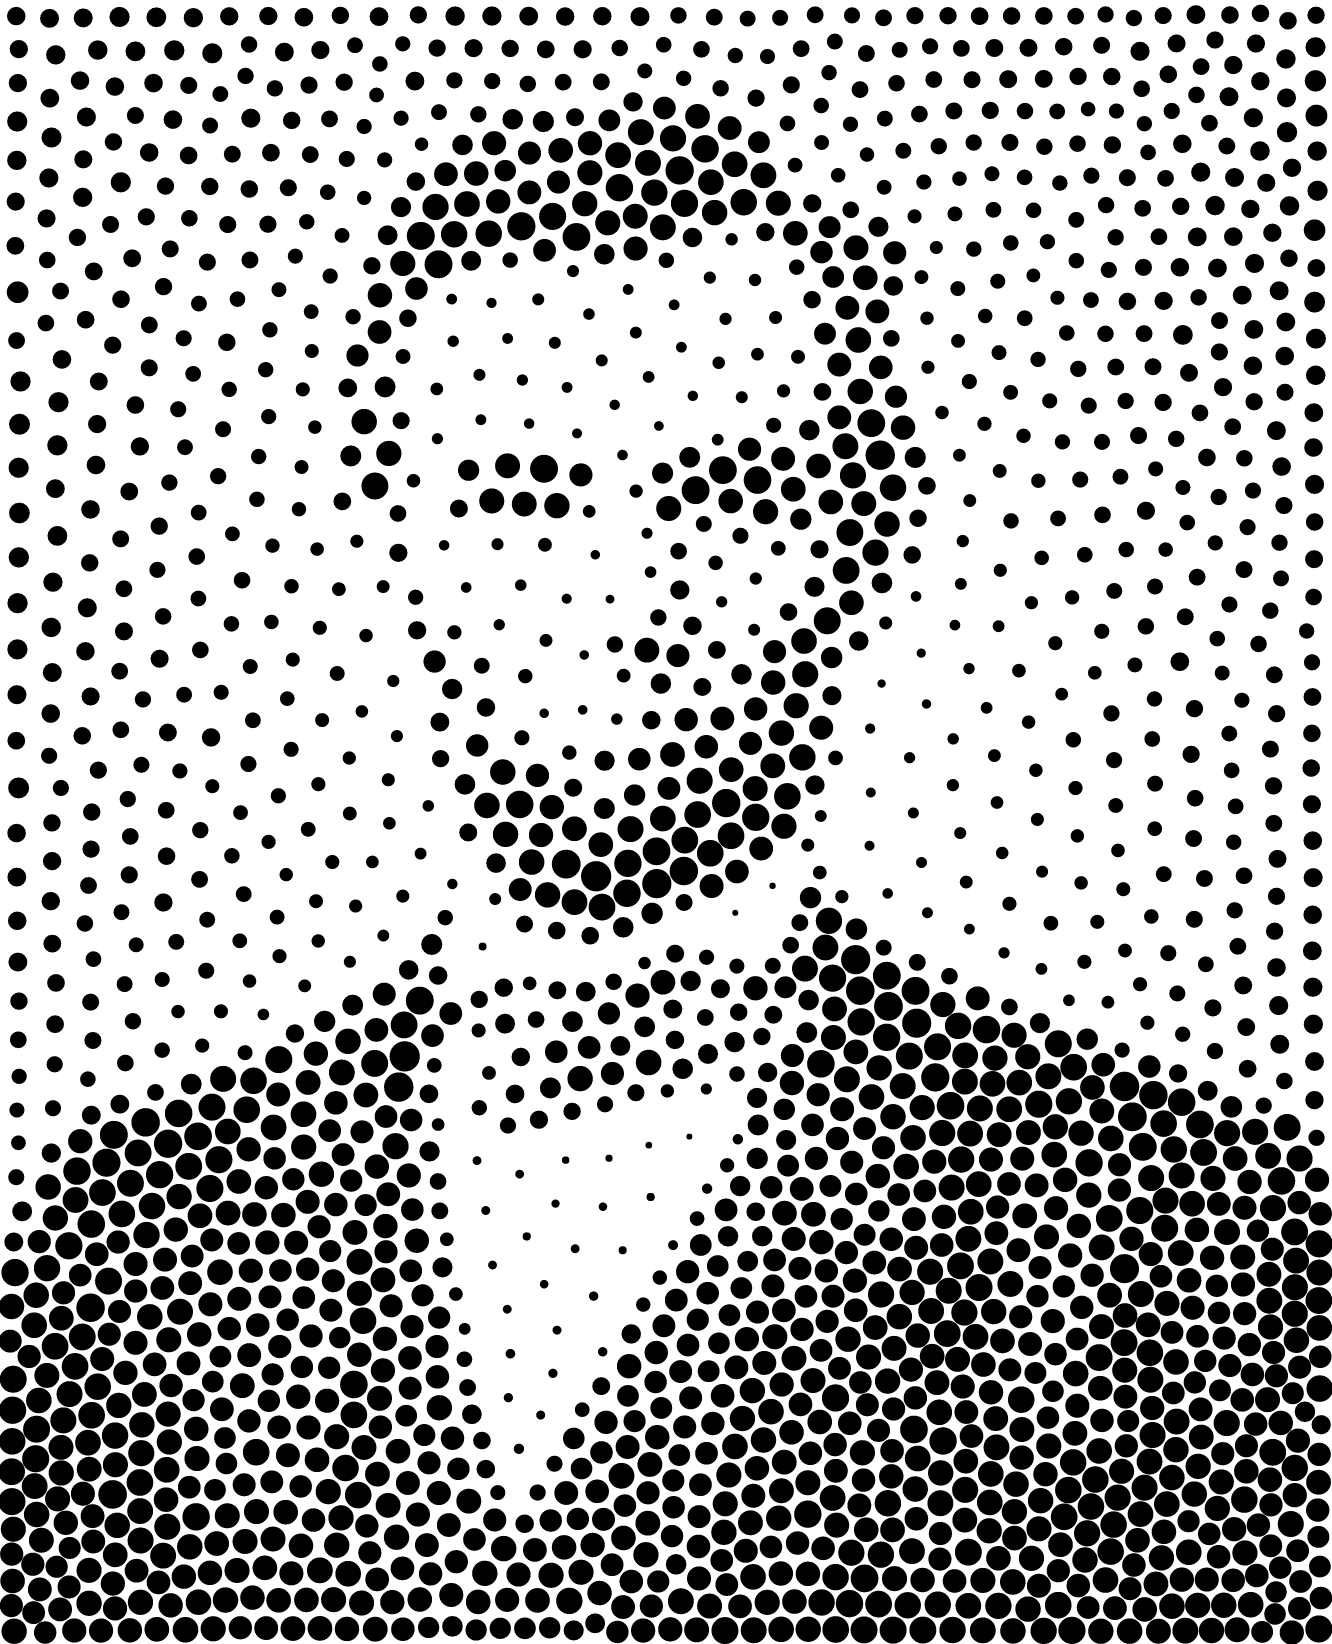
\includegraphics[width=\linewidth]{pix/vr_AL_2000_r10.png}
		\caption{2000px, r=10}
	\end{subfigure}
	\begin{subfigure}[b]{0.2\linewidth}
		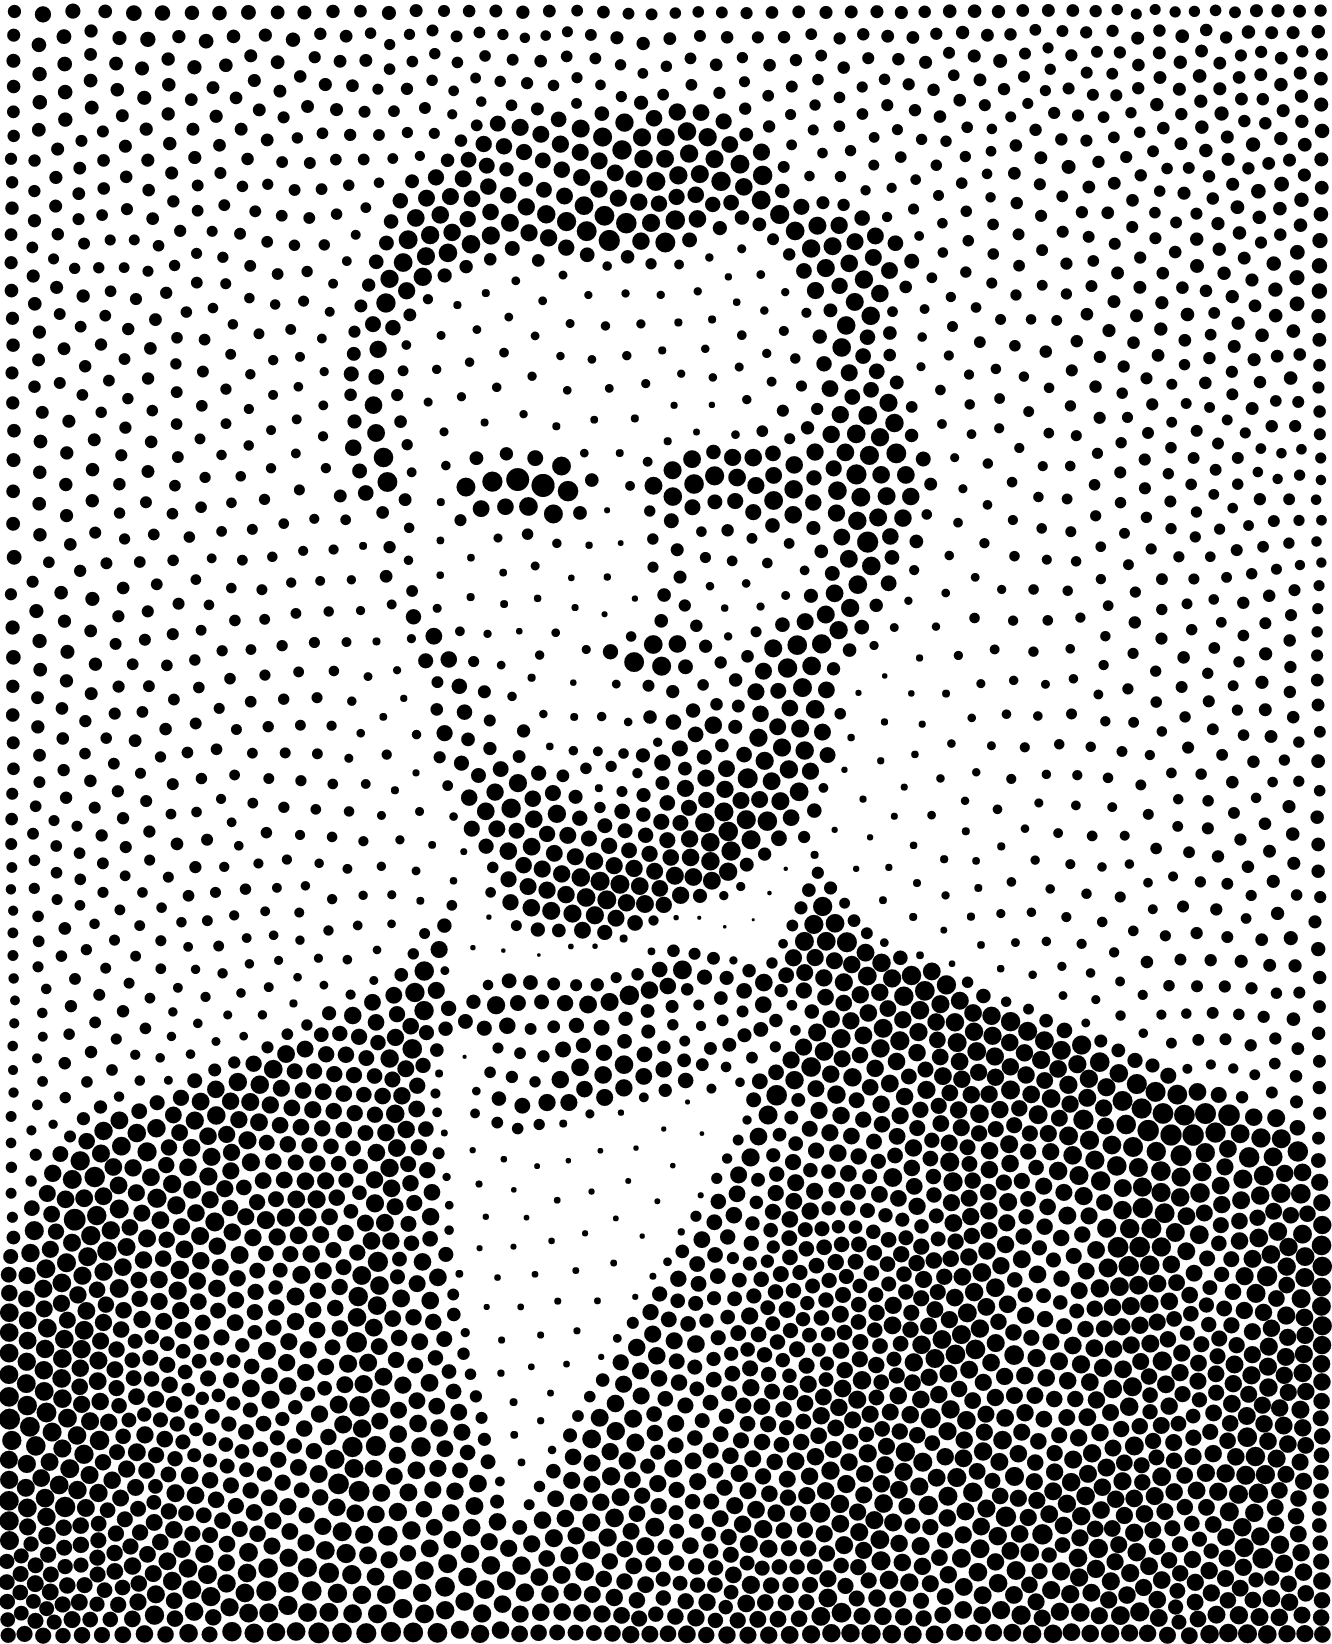
\includegraphics[width=\linewidth]{pix/vr_AL_4000_r10.png}
		\caption{4000px, r=10}
	\end{subfigure}
	\begin{subfigure}[b]{0.2\linewidth}
		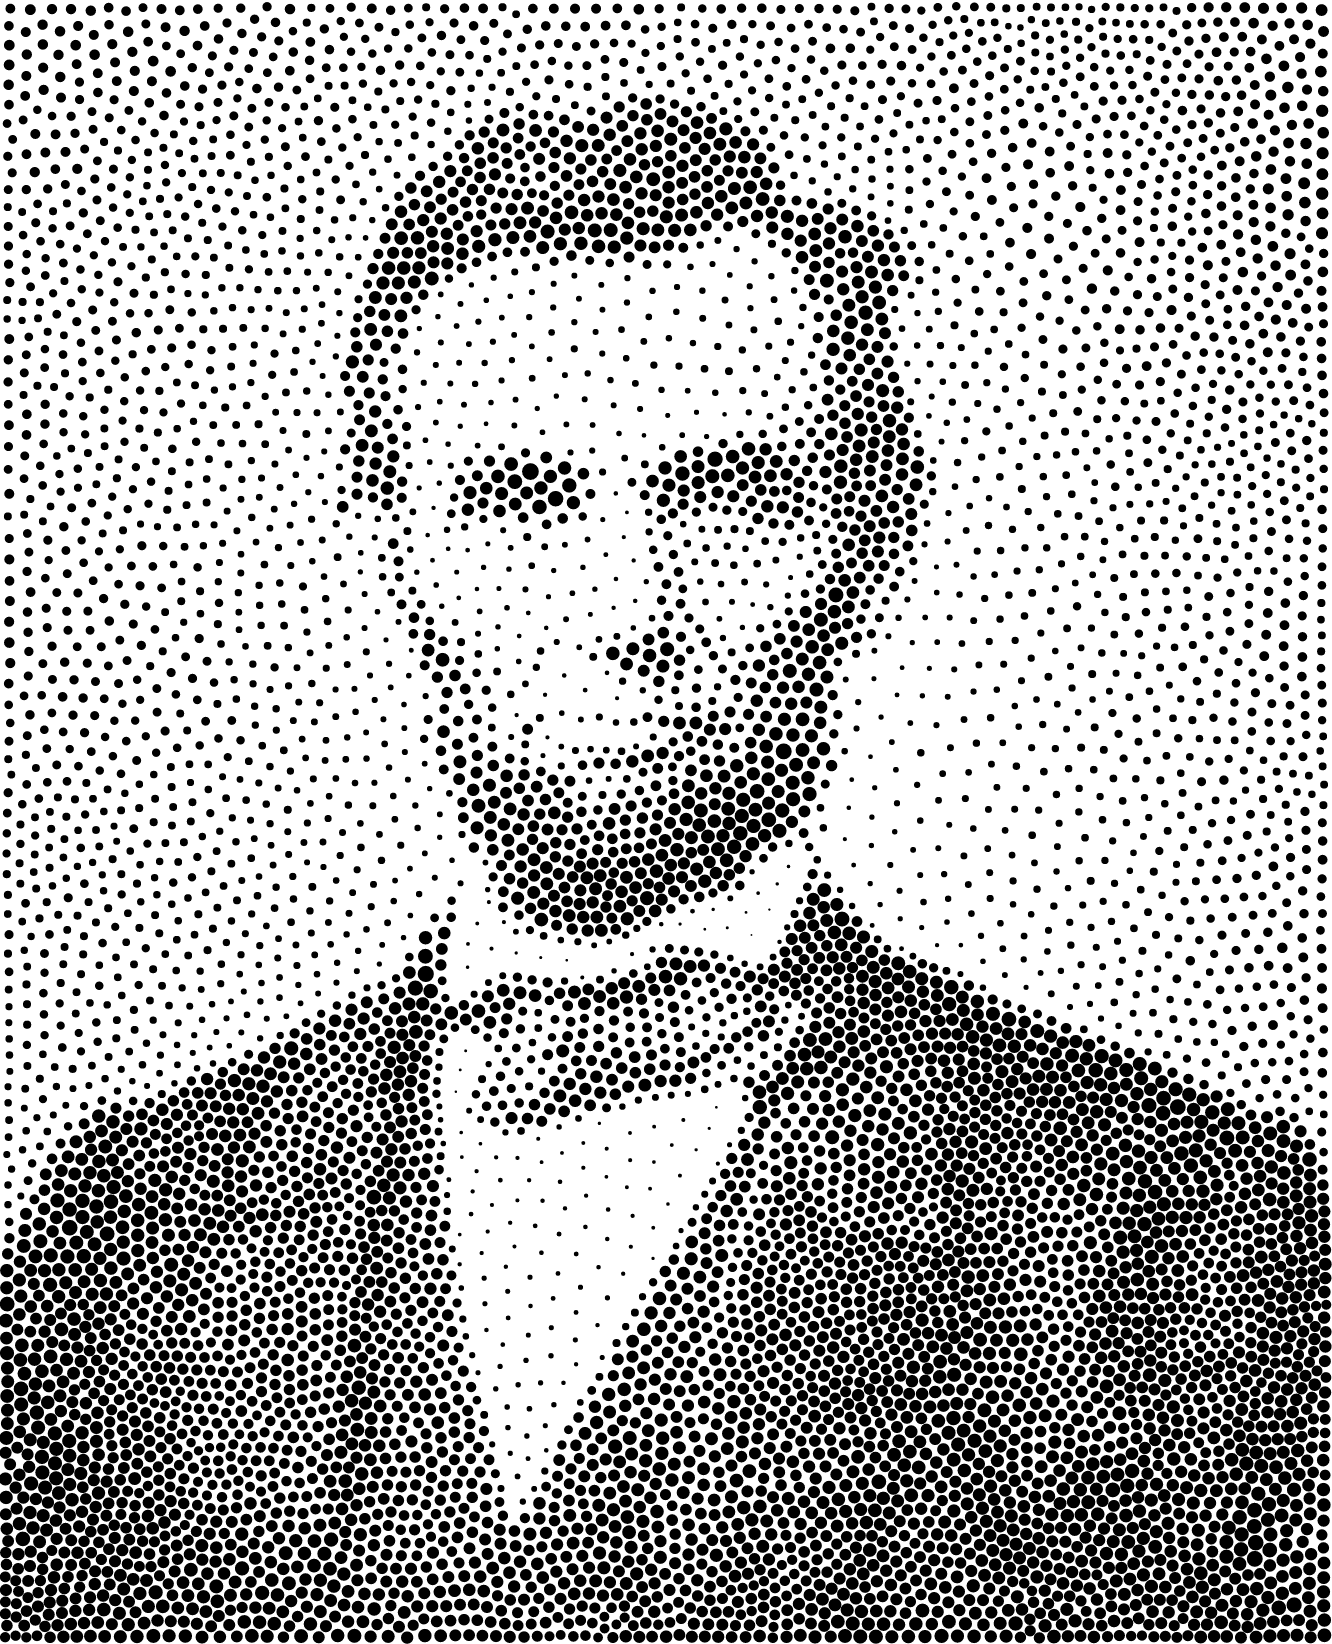
\includegraphics[width=\linewidth]{pix/vr_AL_8000_r10.png}
		\caption{8000px, r=10}
	\end{subfigure}
	\caption{Hedcuter images varying number of disks. Radius = 1.}
	\label{fig:vc_points1}
\end{figure}








\subsection{Variations on Number of Disks}

\subsection{Variations on Speed with Number of Disks}

\subsection{Differences in image type}

\subsection{Differences from WSJ Hedcuts}

\section{Improvement of hedcuter method}

\bibliographystyle{plain}
\bibliography{report}

\end{document}


